\PassOptionsToPackage{hyphens}{url}
\documentclass[11pt]{article}

\usepackage[letterpaper,margin=1in]{geometry}
\usepackage[T1]{fontenc}
\usepackage[utf8]{inputenc}
\usepackage{lmodern}
\usepackage{microtype}
\usepackage{amsmath,amssymb}
\usepackage{booktabs,longtable,array,tabularx}
\usepackage[section]{placeins}
\usepackage{graphicx}
\usepackage[round,authoryear]{natbib}
\usepackage{xcolor}
\usepackage{enumitem}
\usepackage[font=small,labelfont=bf]{caption}
\usepackage[most]{tcolorbox}
\usepackage[colorlinks=true,linkcolor=blue!45!black,citecolor=blue!45!black,urlcolor=blue!45!black]{hyperref}

\setlist{itemsep=2pt,topsep=4pt}
\graphicspath{{generated/}}

% Numbers derived in the text by arithmetic a reader can redo. The build's number
% check skips them; every other decimal must appear in a committed record.
\newcommand{\derived}[1]{#1}

% Named numbers computed from the committed record by `forecast paper-assets`.
% Generated by `forecast paper-assets`. Do not edit by hand.

\newcommand{\BlendHorizon}{46}
\newcommand{\BlendIntervalFiveYears}{[$-0.012$, $+0.169$]}
\newcommand{\BlendIntervalOneMonth}{[$+0.406$, $+0.531$]}
\newcommand{\BlendIntervalOneYear}{[$+0.172$, $+0.311$]}
\newcommand{\BlendIntervalTenYears}{[$-0.093$, $+0.019$]}
\newcommand{\BlendLeadsChain}{17--69}
\newcommand{\BlendMinusChainBelow}{1--8 and 114--120}
\newcommand{\BlendSkillFiveYears}{$+0.097$}
\newcommand{\BlendSkillOneMonth}{$+0.476$}
\newcommand{\BlendSkillOneYear}{$+0.240$}
\newcommand{\BlendSkillTenYears}{$-0.055$}
\newcommand{\BlendSlopeOneYear}{0.870}
\newcommand{\ChainIntervalFiveYears}{[$+0.042$, $+0.119$]}
\newcommand{\ChainIntervalOneMonth}{[$+0.477$, $+0.580$]}
\newcommand{\ChainIntervalOneYear}{[$+0.183$, $+0.312$]}
\newcommand{\ChainIntervalTenYears}{[$+0.009$, $+0.056$]}
\newcommand{\ChainSkillFiveYears}{$+0.088$}
\newcommand{\ChainSkillOneMonth}{$+0.532$}
\newcommand{\ChainSkillOneYear}{$+0.248$}
\newcommand{\ChainSkillTenYears}{$+0.032$}
\newcommand{\ChainSlopeOneYear}{0.933}
\newcommand{\FirstForecastMonth}{March 1994}
\newcommand{\ForecastCount}{11,730}
\newcommand{\ForecastDates}{391}
\newcommand{\IndependentObservationsFiveYears}{5.5}
\newcommand{\IndependentObservationsOneMonth}{32.4}
\newcommand{\IndependentObservationsOneYear}{31.5}
\newcommand{\InflationAfterSurge}{0.880}
\newcommand{\InflationAverageBeforeSurge}{0.266}
\newcommand{\InflationBeforeSurge}{0.136}
\newcommand{\LastForecastMonth}{September 2026}
\newcommand{\ModelHorizon}{29}
\newcommand{\ModelIntervalFiveYears}{[$-0.121$, $+0.191$]}
\newcommand{\ModelIntervalOneMonth}{[$+0.161$, $+0.369$]}
\newcommand{\ModelIntervalOneYear}{[$+0.102$, $+0.258$]}
\newcommand{\ModelIntervalTenYears}{[$-0.301$, $-0.040$]}
\newcommand{\ModelMinusChainBelow}{1--16 and 103--120}
\newcommand{\ModelSkillFiveYears}{$+0.069$}
\newcommand{\ModelSkillOneMonth}{$+0.290$}
\newcommand{\ModelSkillOneYear}{$+0.179$}
\newcommand{\ModelSkillTenYears}{$-0.211$}
\newcommand{\ModelSlopeOneYear}{0.613}
\newcommand{\RecessionAfterTwoThousandOne}{0.639}
\newcommand{\RecessionDuringTwoThousandOne}{0.166}
\newcommand{\ResolvedCount}{9,702}


\newtcolorbox{keybox}[1]{colback=blue!3!white,colframe=blue!40!black,boxrule=0.6pt,
  arc=2pt,left=8pt,right=8pt,top=5pt,bottom=5pt,fonttitle=\bfseries\small,fontupper=\small,
  title={#1}}
\newtcolorbox{plainbox}[1]{colback=black!2!white,colframe=black!45,boxrule=0.5pt,
  arc=2pt,left=8pt,right=8pt,top=6pt,bottom=6pt,fonttitle=\bfseries,title={#1}}

\title{When to Ship the Historical Average:\\[2pt]
\large A Pre-Registered, Point-in-Time Test of Regime-Based Probability Forecasts for the US Economy}
\author{Jeddy Xie\thanks{Correspondence: \texttt{xiejeddy@gmail.com}. Code, data registries,
pre-registrations and every result in this paper:
\url{https://github.com/Jeddy-Xie/forecasting-the-future}.}}
\date{29 September 2026}

\begin{document}
\maketitle

\begin{abstract}
\noindent
How far ahead can probability forecasts of the US economy beat the historical average? We forecast ten
yes-or-no events (recession, inflation, interest-rate, unemployment, yield-curve and output thresholds)
from a hidden Markov model with separate regime chains for growth and for inflation with interest rates.
The model uses only data published by each forecast date, is walked forward over 391 months from 1994 to 2026, and is
judged by acceptance rules committed before any result was seen. Scored at every horizon from 1 to 120
months, the regime model beats the historical average for 29 months. A forecaster with no regimes, which
tracks only whether each condition holds now, does at least as well at every horizon: most of the skill
is persistence. An equal blend of the two, adopted in a pre-registered experiment, beats the average for
46 months. At one year it removes on average about a quarter of the average's squared error and passes
every acceptance gate. Beyond about four years we ship the average. We document how look-ahead leaks and
an accidentally weak benchmark had inflated earlier estimates. Because every choice was made on one
sample, we register forecasts forward as the only out-of-sample test.
\end{abstract}

\noindent\textbf{Keywords:} probability forecasting; hidden Markov models; regime switching; Brier skill
score; forecast evaluation; pre-registration; real-time data; persistence\\
\noindent\textbf{JEL codes:} C22, C53, E32, E37

\begin{keybox}{Key findings, in plain language}
\begin{enumerate}[leftmargin=*]
\item \textbf{One year ahead, the forecasts are clearly better than the historical average.} Across the ten
  questions they remove on average about a quarter of the average's error (Brier skill
  \BlendSkillOneYear, 90\% interval \BlendIntervalOneYear).
\item \textbf{The advantage fades with the horizon.} The forecast that ships beats the average for about
  four years (\BlendHorizon{} months); the regime model on its own, for about two and a half
  (\ModelHorizon{} months). Past that, the honest forecast is the historical average.
\item \textbf{Most of the skill is persistence: knowing where the economy is now.} A simple forecaster
  with no regimes, which only tracks whether each condition currently holds, does at least as well as the
  regime model at every horizon from one month to ten years.
\item \textbf{Regimes add information where the model observes the question} (inflation, and interest
  rates near zero), and not for recessions or unemployment, which it never observes.
\item \textbf{The forecasts react to turning points; they do not anticipate them.} They rose sharply once
  the 2021 inflation surge showed up in published data, and they registered the 2001 recession only
  after it had ended.
\item \textbf{Honesty was expensive.} Closing look-ahead leaks, and later adopting a fair benchmark, each
  took the model's one-year verdict away; each time, a pre-registered improvement earned it back.
\end{enumerate}
\end{keybox}

\section{Introduction}\label{sec:introduction}

Households, firms and public institutions make decisions that depend on questions such as \emph{will
there be a recession within the next year?} or \emph{will inflation be above three percent a year from
now?} Useful answers to such questions are probabilities, not point predictions, and the obvious default
answer is the historical average: how often the event has happened in the past. A forecasting method is
worth its complexity only if it beats that default, and a forecaster should know the horizon beyond
which it no longer does.

This paper asks, for ten binary questions about the US economy, how far ahead that horizon lies. The
forecasts come from a hidden Markov model \citep{hamilton1989new,rabiner1989tutorial}: the economy is
assumed to move between a small number of persistent, unobserved \emph{regimes}, each with its own
typical growth, inflation and interest rates. The model infers which regime the economy is probably in
today, projects that forward, and converts the projection into a probability for each question.

Three difficulties make an honest answer hard to obtain, and much of this paper is about meeting them.

\emph{Look-ahead.} A backtest that uses any information not available on the forecast date overstates
skill without announcing it. Economic data are revised after publication, recessions are dated months or
years after the fact, and fitting choices made on the full sample carry the future into the past. We
build every training panel from data as it was published \citep{croushore2001realtime}, date recession
status by the announcements that settled it \citep{nber2026announcements}, and test all of this with an
executable audit that perturbs everything a forecast should not know and requires the forecast not to
change.

\emph{The benchmark.} A skill score is only as meaningful as its reference. We found that our original
reference, the average of every outcome since each data series began, reached back to 1854 for
recession dating while the model learned only from 1950 onward, and that a simple forecaster without
regimes beat the model at one year. Both findings changed the conclusions of this paper, and both are
reported.

\emph{Small samples.} Thirty-two years of monthly forecasts sound like a lot of data. Because forecasts
made in consecutive months share most of their future, the one-year results rest on about 31
independent observations and the five-year results on about 5.5. Every interval in this paper accounts
for that, and we say where the data cannot answer.

\paragraph{Contributions.} First, we measure the skill of regime-based probability forecasts against the
historical average at every horizon from 1 to 120 months, under acceptance rules committed before the
first backtest ran, and read off the horizon beyond which the average should ship: \ModelHorizon{} months
for the regime model and \BlendHorizon{} months for the blend that ships. Second, we show that a
regime-free forecaster that knows only whether each condition holds now matches or beats the regime model
at every horizon, locate the questions on which regimes do add information, and adopt, through a
pre-registered experiment, an equal blend of the two that passes every acceptance gate at one year.
Third, we document the evaluation itself: three look-ahead paths and an accidentally weak benchmark, how
each was found, and what each correction did to the headline number. Fourth, we release a deterministic,
tested and audited implementation, and register its forecasts forward every month, so that the claims
here will be tested on data that did not exist when they were made.

\paragraph{Related literature.} Regime-switching models of the business cycle go back to
\citet{hamilton1989new}; \citet{kim1999statespace} and \citet{hamilton2016macroeconomic} survey the
econometrics, and \citet{ang2012regime} their use in finance. Our two-chain model is a factorial hidden
Markov model \citep{ghahramani1997factorial}, fitted by expectation maximisation
\citep{baum1970maximization,dempster1977maximum}. A long line of work finds that regime-switching models
often forecast no better than simple alternatives \citep{clements1998comparison,dacco1999why}, which
agrees with what we find against a persistence benchmark; the broader forecasting literature reports
that simple methods and combinations are hard to beat \citep{bates1969combination,timmermann2006forecast,
makridakis2018m4}. We score forecasts with the Brier score \citep{brier1950verification}, a strictly
proper scoring rule \citep{gneiting2007strictly}, and its skill score against a reference
\citep{murphy1973new,murphy1988skill}; comparisons use paired differences in the spirit of
\citet{diebold1995comparing}, with moving-block bootstrap intervals for dependent data
\citep{kunsch1989jackknife,efron1979bootstrap}. Recession forecasting has focused on the yield curve
\citep{estrella1998predicting,estrella2006yield,rudebusch2009forecasting} and on real-time dating
\citep{chauvet2008comparison}; the value of real-time data for honest evaluation is established by
\citet{croushore2001realtime}. Our use of pre-registration follows \citet{nosek2018preregistration}, and
our concern with searching over many specifications follows \citet{white2000reality} and
\citet{harvey2016cross}.

\paragraph{Roadmap.} Section~\ref{sec:primer} is a short primer for readers without a background in
forecasting or economics. Section~\ref{sec:data} describes the questions and the data,
Section~\ref{sec:model} the model, and Section~\ref{sec:evaluation} the evaluation design and the rules
committed in advance. Section~\ref{sec:results} presents the results, Section~\ref{sec:discussion}
discusses what they mean and what they cannot show, and Section~\ref{sec:conclusion} concludes. The
appendices hold a glossary, the full decision rules, and every table behind the figures.

\section{A primer for readers new to forecasting}\label{sec:primer}

\paragraph{Probability forecasts and how to score them.} A probability forecast says how likely an event
is, for example ``a 30\% chance of a recession within the next year''. A single forecast cannot be right
or wrong, but many can be scored. The \emph{Brier score} is the average squared distance between the
forecast probability $p$ and what happened, $y = 1$ if the event occurred and $0$ if not:
\begin{equation}
  \text{Brier} = \frac{1}{N}\sum_{i=1}^{N} (p_i - y_i)^2 .
\end{equation}
Lower is better. A forecast of \derived{0.9} for an event that happens scores \derived{0.01}; a forecast of
\derived{0.9} for one that does not scores \derived{0.81}. The Brier score rewards forecasts that are
confident when they should be and cautious when they should be, and it cannot be gamed by shading
probabilities away from what the forecaster believes \citep{gneiting2007strictly}.

\paragraph{Skill against a benchmark.} To ask whether a forecaster is useful we compare it with a simple
reference that anyone could produce. The \emph{Brier skill score} is
\begin{equation}
  \text{skill} = 1 - \frac{\text{Brier of the forecaster}}{\text{Brier of the reference}} .
\end{equation}
A skill of zero means no better than the reference, a skill of one would be perfect, and a negative skill
means worse than the reference. A skill of \BlendSkillOneYear{} means the forecaster's squared error is
about three quarters of the reference's.

\paragraph{Two simple references.} The first is the \emph{historical average}: the fraction of past
occasions on which the question resolved yes, using only outcomes that were known on the forecast date.
The second, less familiar, is \emph{persistence}. Most economic conditions are sticky: if unemployment is
above seven percent this month, it very probably will be next month. A forecaster that knows only
whether each condition holds now, and how often such conditions have started and stopped in the past,
can be hard to beat at short horizons. We call it the \emph{condition chain}.

\paragraph{Regimes and hidden Markov models.} The idea behind a regime model is that the economy spends
long stretches in recognisable states (steady growth with low inflation; contraction; high inflation with
high interest rates) and switches between them occasionally. The states are not observed; they are
inferred from data such as output growth, inflation and interest rates. A hidden Markov model makes this
precise: each regime has a typical pattern of observations, and each month the economy either stays in
its regime or moves to another with fixed probabilities. Given data up to today, the model gives the
probability of being in each regime today and, by applying those switching probabilities repeatedly, in
each regime at any future date.

\paragraph{Why a long sample holds few observations.} A one-year forecast made in January and one made in
February share eleven months of the future they are about, so they are far from independent. Over
long horizons this overlap dominates: our 391 monthly forecast dates are worth about
\IndependentObservationsOneYear{} independent observations at one year and \IndependentObservationsFiveYears{}
at five years. That is why the uncertainty intervals in this paper widen so fast with the horizon, and why
we treat anything beyond five years as uninformative.

\section{Questions, horizons and data}\label{sec:data}

\paragraph{The ten questions.} Every question asks whether a monthly condition holds, either in the
single month at the horizon (\emph{at the horizon}) or in at least one month between now and the horizon
(\emph{any time}). Table~\ref{tab:questions} lists them. Each is asked at horizons of one, five and ten
years, and scored at every horizon from 1 to 120 months in Section~\ref{sec:horizon}. Restricting every
question to a condition on a single month is what lets one set of per-regime rates serve every
horizon (Section~\ref{sec:composition}).

\begin{table}[t]
\centering
\caption{The ten questions. \emph{Any time} questions ask whether the condition holds in at least one
month between the forecast date and the horizon; \emph{at the horizon} questions ask about the horizon
month alone. The last column says whether the model observes the question's series directly.}
\label{tab:questions}
\small
\begin{tabular}{p{0.42\linewidth}lll}
\toprule
Question & Series & Kind & Model observes it? \\
\midrule
Year-over-year consumer price inflation above 5\% & CPIAUCSL & any time & yes \\
Year-over-year consumer price inflation above 3\% & CPIAUCSL & at the horizon & yes \\
Effective federal funds rate below 1\% & FEDFUNDS & any time & through the bill rate \\
Effective federal funds rate above 4\% & FEDFUNDS & at the horizon & through the bill rate \\
Ten-year Treasury yield below the three-month bill rate & GS10, TB3MS & any time & one leg \\
Industrial production growing more than 2\% a year & INDPRO & at the horizon & yes \\
Unemployment rate above 7\% & UNRATE & any time & no \\
Unemployment rate above 5\% & UNRATE & at the horizon & no \\
Economy in a recession dated by the NBER & USREC & any time & no \\
Economy in a recession dated by the NBER & USREC & at the horizon & no \\
\bottomrule
\end{tabular}
\end{table}

\paragraph{What the model observes.} The model sees three monthly series: year-over-year growth of
industrial production (INDPRO), year-over-year consumer price inflation (CPIAUCSL), and the three-month
Treasury bill rate (TB3MS), all from the Federal Reserve Bank of St.\ Louis
\citep{stlouisfed2026fred,stlouisfed2026alfred}. The bill rate stands in for the policy rate because it
is one continuous series back to 1934. Growth and inflation enter as year-over-year log changes, which
makes vintages published on different index bases comparable. Each column is standardised with an
expanding window, so no month is scaled using information from a later one.

\paragraph{Data as it was published.} Every training panel is assembled \emph{as of} a forecast date.
Series that are revised after publication (output and prices) are read from archival vintages
\citep{stlouisfed2026alfred}: the version of the series that existed on that date. Market rates, which
are never revised, are censored by their publication lag. The archive's consumer price vintages are
usable only from March 1994; before then it returns a rolling window of about nineteen observations. The
walk-forward therefore starts in March 1994, the first month in which every input is genuinely point in
time. The conditions from which the model learns its per-regime rates are read from final data, with
publication timing enforced (Section~\ref{sec:discussion} measures the difference). Recession status is published only when the National Bureau of Economic Research announces the
turning point that settles it \citep{nber2026cycles,nber2026announcements}, between four months and almost
two years after the fact; a month's recession code counts as known at the later of a fixed 400-day lag
and that announcement.

\paragraph{Sample.} The regime model is fitted on months from December 1950. The number of regimes is
chosen once, on the 518 months up to January 1994, before any forecast is scored. Forecasts are issued
monthly from \FirstForecastMonth{} to \LastForecastMonth: \ForecastDates{} forecast dates, and
\ForecastCount{} forecasts across questions and horizons, of which \ResolvedCount{} had resolved when
this paper was written.

\section{The model}\label{sec:model}

\subsection{Two regime chains}

Let $y_t = (g_t, \pi_t, r_t)$ be standardised growth, inflation and the bill rate in month $t$. A single
hidden Markov chain over all three columns, the model we began with, is pulled onto the slow clock of
inflation and rates: its regimes last years, while output growth on its own switches about three times
as fast. We therefore use two independent chains \citep{ghahramani1997factorial}. A growth chain
$S^{g}_t \in \{1,\dots,K_g\}$ drives growth, and a levels chain $S^{\ell}_t \in \{1,\dots,K_\ell\}$ drives
inflation and rates:
\begin{equation}
  g_t \mid S^{g}_t = i \;\sim\; \mathcal{N}(\mu^{g}_i, \sigma^{2}_i), \qquad
  (\pi_t, r_t) \mid S^{\ell}_t = j \;\sim\; \mathcal{N}(\mu^{\ell}_j, \Sigma_j),
\end{equation}
with transition matrices $A^{g}$ and $A^{\ell}$. The joint regime is the pair $s = (i, j)$, its transition
matrix is the Kronecker product $A = A^{g} \otimes A^{\ell}$, and its emission log density is the sum of
the two blocks'. Over the product space this is an ordinary Gaussian hidden Markov model with
$K_g K_\ell$ states, so filtering and projection are standard, and it is fitted exactly by expectation
maximisation because the complete-data likelihood separates by chain. The model is written out rather
than imported so that the backtest can use \emph{filtered} probabilities, which condition only on data
up to the forecast date, and never smoothed ones, which condition on the whole sample.

\paragraph{How many regimes.} Each chain's number of states is chosen from one to four, once, on the
burn-in window, by a fixed rule: a candidate is disqualified if any of its states has an expected visit
shorter than three months or holds under five percent of months; among the rest, held-out log likelihood on the
last fifth of the window decides, with the Bayesian information criterion \citep{schwarz1978estimating}
reported beside it. Both chains chose four states, so the model has sixteen joint regimes on 58 free
parameters. An unrestricted sixteen-state chain would need 399, and our own selection rule rejects one:
some of its regimes hold under five percent of months, too few to estimate anything from. Fits use twenty
random restarts, and every walk-forward refit happens once a year.

\subsection{From regimes to probabilities}\label{sec:composition}

For each question and regime $k$ the model learns three rates from the training window, weighting each
month by the filtered probability of regime $k$: the \emph{occupancy} $o_k$, how often the condition
holds in regime $k$; the \emph{entry hazard} $e_k$, how often it starts to hold after a month in which it
did not; and the \emph{persistence} $p_k$, how often it keeps holding. Each is shrunk toward its pooled
value by a Beta prior of strength ten, so a rarely visited regime borrows strength from the rest.

Let $\alpha_t$ be the filtered regime distribution on the forecast date. An \emph{at the horizon}
question is answered by projecting the regimes forward and averaging the occupancies:
$P(C_{t+h} = 1) = \alpha_t A^{h} o$. An \emph{any time} question is answered through the probability of
surviving the whole window without the condition. The first month uses the persistence if the
condition holds now and the entry hazard if not; every later month is reached only along paths on which
it has not held, so the entry hazard applies throughout:
\begin{equation}
  P(\text{holds in some month } 1..h) = 1 - \alpha_t\, A D_1 \,(A D_e)^{h-1} \mathbf{1},
\end{equation}
where $D_e = \operatorname{diag}(1 - e)$ and $D_1$ is $\operatorname{diag}(1-p)$ or $\operatorname{diag}(1-e)$
according to today's condition, and $A D$ scales each column of $A$.

\subsection{The condition chain and the blend}\label{sec:blend}

The condition chain is the same construction with a single regime: a two-state Markov chain on each
question's own monthly condition, with an entry hazard and a persistence estimated by plain counts from
every condition published by the forecast date since the model's sample began, re-estimated every month.
It starts from the last
published value of the condition, steps through the months until the forecast date (a month or two for
most series, more than a year for recession dating), and then through the horizon. It knows nothing
about growth, inflation or rates beyond the question's own series.

The forecast that ships is the equal-weight blend,
\begin{equation}
  p^{\text{blend}} = 0.5\, p^{\text{regime model}} + 0.5\, p^{\text{condition chain}},
\end{equation}
at every question and horizon. The weight was fixed at one half in the experiment's registration and is
never fitted.

\section{Evaluation design}\label{sec:evaluation}

\subsection{Rules committed before the results}

The project's first decision rule, \emph{rule 0001}, was committed on 8 September 2026 before any
backtest had run. At each horizon it ships the model only if five gates all hold, and otherwise ships
the historical average and records which gate failed. Table~\ref{tab:gates} lists the gates. The
thresholds were chosen from the structure of the problem rather than from data: a skill below 0.02 is not
worth the machinery, two positive sub-periods out of four is a coin flip, and at a total variation
distance below 0.05 a projection can no longer be told apart from the long-run regime distribution. The
same rule stated its expected outcome in advance: \emph{``One year passes. Five years is marginal. Ten
years fails.''}

\begin{table}[t]
\centering
\caption{The five acceptance gates. Rule 0001 was committed before the first backtest and is frozen;
rule 0007 keeps its thresholds, changes the benchmark and the calibration test, and adds the condition
chain as a bar to clear. Both verdicts are always reported.}
\label{tab:gates}
\small
\begin{tabular}{p{0.16\linewidth}p{0.38\linewidth}p{0.38\linewidth}}
\toprule
Gate & Rule 0001 (8 September 2026) & Rule 0007 (29 September 2026) \\
\midrule
Skill & Mean Brier skill across the questions above 0.02, and its 90\% interval above zero, against
the average since each series began & The same against R1, the average over the model's own sample;
pooled skill must agree in sign \\
Calibration & Ten-bin calibration error below 0.10 and no reversal beyond noise & Logistic
recalibration slope interval contains one (Section~\ref{sec:calibration}) \\
Robustness & Skill positive in at least three of four chronological sub-periods & Same, against R1 \\
Honesty & Projected regime distribution at least 0.05 from the stationary one & Same \\
Regimes exist / chain & More than one regime beats one on held-out likelihood and the criterion &
Model minus the condition chain not entirely below zero at 90\% \\
\bottomrule
\end{tabular}
\end{table}

\paragraph{Why a successor rule, and what it cannot claim.} Rule 0001 names the historical average but
not where its window starts, and the archive chose it: back to 1854 for recession dating and 1919 for
industrial production, while the model learns only from 1950. That weak reference flattered every skill
score. Rule 0001 also never asked whether regimes beat a forecaster without them. A review of the
project on 25 September 2026 measured both problems, and \emph{rule 0007}, registered on 29 September
2026, makes the fairer reference (R1) and the condition chain (R2) the standard for every new claim. Rule
0007 was written after its motivating numbers had been seen, and its registration says so; what it fixes
in advance is how every later experiment and re-release is read. Rule 0001 stays frozen and its verdicts
are printed beside rule 0007's.

\subsection{Intervals and effective sample size}

Differences in mean skill are computed on the same forecasts for both forecasters. Intervals come from a
moving-block bootstrap over forecast dates \citep{kunsch1989jackknife}, with blocks at least as long as
the horizon (and at least twelve months), 10,000 resamples and a fixed seed, so that each resample keeps
the dependence between overlapping forecasts. The effective number of independent observations reported
beside each estimate is the number of forecast dates whose outcomes have resolved, divided by the block
length.

\subsection{Calibration}\label{sec:calibration}

A forecast is \emph{calibrated} if events it calls 30\% likely happen about 30\% of the time. Rule
0001's ten-bin calibration error turned out to be unusable at this sample size: a perfectly calibrated
forecaster with about 31 independent observations fails it about 91\% of the time. Rule 0007 instead fits
a logistic recalibration \citep{cox1958two}, $\operatorname{logit} P(y = 1) = a + b \operatorname{logit}
p$, where a calibrated forecaster has slope $b = 1$. Before using it, we simulated its size on 200
panels shaped like the one-year sample: a perfectly calibrated forecaster passed the joint test on
$a$ and $b$ only 60.5\% of the time and the slope test alone 77.5\% of the time, so the registration's
pre-stated fallback, the slope alone, applies. It still errs against shipping the model about one time
in four, and we report that rather than adjust for it. A slope below one means the forecaster is
overconfident: its probabilities should be pulled toward the middle.

\subsection{The information horizon}

Because the regime chain mixes, the projected regime distribution approaches the chain's long-run
(stationary) distribution as the horizon grows, at a rate set by the transition matrix's second largest
eigenvalue. Once the two are closer than 0.05 in total variation, a regime forecast is the unconditional
base rate in disguise, and rule 0001's honesty gate refuses to ship it as a prediction. For the current
fit the growth chain's second eigenvalue is 0.946 and the levels chain's 0.983, a half-life of about 39
months for the joint chain; the mean distance to the stationary distribution is 0.486 at one year, 0.121
at five years and 0.033 at ten.

\subsection{Guarding against look-ahead}\label{sec:audit}

Three guards run on every change. The first is structural: every function that assembles a training
panel requires an as-of date, standardisation windows only expand, and backtests use filtered
probabilities. The second is an executable audit: it takes a cutoff date, replaces everything that was
not available at the cutoff with perturbed values, re-runs the walk-forward, and requires every forecast
issued on or before the cutoff to come out byte for byte identical. It runs at two cutoffs, March 2000
and March 2022; the second reaches every recession announcement since 1991. The third is an independent
reviewer, who did not write the change, looking for any path by which later information reaches a
forecast. Section~\ref{sec:honesty} reports what these guards found.

\subsection{Skill at every horizon}\label{sec:horizon-rule}

To answer the question in the title, measurement 0010 scored the forecasts at every horizon from 1 to 120
months, under a reading rule registered before it ran. A forecaster \emph{carries skill} at a horizon if
its mean skill against R1 exceeds 0.02 and its 90\% interval lies above zero. The \emph{ship-the-average
horizon} is the last month up to which it carries skill without a break. Horizons with fewer than 5.5
effective independent observations, which here means beyond 60 months, are drawn but labelled
uninformative.

\subsection{Experiments and multiple comparisons}

Every attempt to improve the model was run as a pre-registered experiment: hypotheses, hyperparameters,
predictions and the decision rule were committed before any arm was implemented. Each arm ran in its own
copy of the repository against a fixed reference, together with a control arm that must reproduce the
reference exactly. With three competing arms, each is judged at a family-wise 90\% level, that is a
96.67\% interval \citep{dunn1961multiple}; with six, at 98.33\%. An arm is \textsc{confirmed in sample} if
its one-year interval at that level lies entirely above zero. It is \textsc{harmful} if at any horizon
its 90\% interval lies entirely below $-0.02$, and void unless both the audit and an independent review
pass. Adoption needs a confirmed arm that is neither harmful nor void, and a separate recorded decision.
``In sample'' is the ceiling: every arm was designed by someone who had already seen the reference's
results on this sample.

\subsection{Decisions made by delegation}\label{sec:delegation}

On 29 September 2026 the author delegated the project's open research decisions to an AI model
(claude-fable-5-1), briefed in writing with the evidence, the house rules and numbered questions. Its
twenty-one decisions, among them registering rule 0007, approving experiment 0008, adopting the blend and
re-releasing the forecasts, are recorded verbatim with their reasons in the repository. They are labelled
throughout as delegated rather than as the author's own judgement, and any of them can be reversed. Where
executing a decision required a deviation, the deviation is recorded beside it.

\section{Results}\label{sec:results}

\subsection{The verdict}

Table~\ref{tab:verdict} gives the verdict for the forecast that ships, the blend, under both rules. At
one year both rules ship the blend: its skill against R1 is \BlendSkillOneYear{} with 90\% interval
\BlendIntervalOneYear, its calibration slope is \BlendSlopeOneYear{} with interval [0.603, 1.198], it is
positive in all four sub-periods, and the condition chain does not beat it. At five and ten years both
rules ship the historical average.

\begin{table}[t]
\centering
\caption{The verdict for the blend (configuration \texttt{7647c129be85291e}) under both rules. Skill is
the mean Brier skill across the ten questions, with its 90\% moving-block bootstrap interval.}
\label{tab:verdict}
\small
\begin{tabular}{lllrl}
\toprule
Horizon & Rule & Verdict & Skill [90\% interval] & Gates failed \\
\midrule
1 year & 0001 & ship the model & $+0.3201$ [$+0.2219$, $+0.4134$] & none \\
1 year & 0007 & ship the model & $+0.2401$ [$+0.1715$, $+0.3113$] & none \\
5 years & 0001 & ship the average & $+0.1447$ [$+0.0050$, $+0.2311$] & calibration \\
5 years & 0007 & ship the average & $+0.0970$ [$-0.0120$, $+0.1691$] & skill, calibration, robustness \\
10 years & 0001 & ship the average & $-0.0062$ [$-0.0477$, $+0.0891$] & skill, calibration, honesty \\
10 years & 0007 & ship the average & $-0.0548$ [$-0.0928$, $+0.0194$] & skill, honesty, the chain \\
\bottomrule
\end{tabular}
\end{table}

The gap between the two rules' one-year skill, $+0.3201$ against $+0.2401$, is entirely the benchmark:
the same forecasts look better against an average that reaches back to 1854.

\subsection{How far ahead: when to ship the average}\label{sec:horizon}

Figure~\ref{fig:curves} shows skill against R1 at every horizon for the three forecasters, and
Table~\ref{tab:curve} reads it at selected months; Appendix~\ref{app:every-month} lists every month.

\begin{figure}[t]
\centering
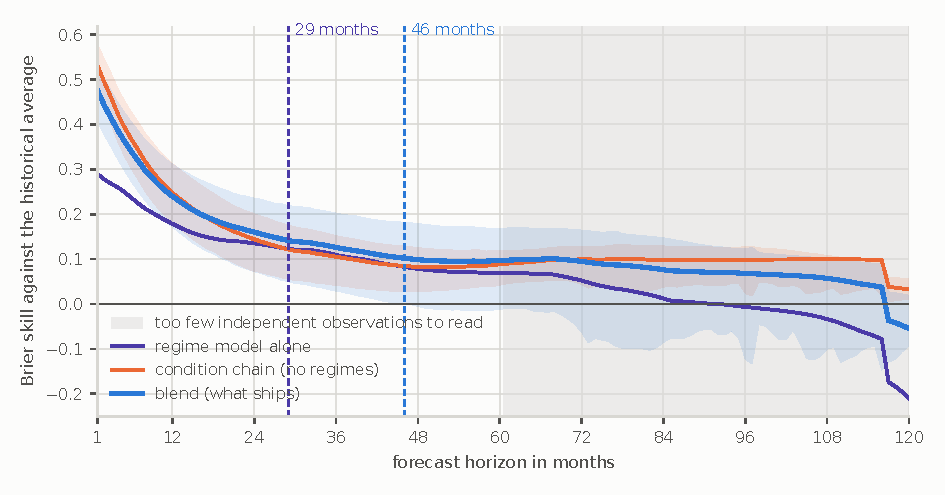
\includegraphics[width=\linewidth]{skill_curves.pdf}
\caption{Brier skill against the historical average (R1) at every horizon from 1 to 120 months, with 90\%
bands for the blend and the condition chain. Dashed lines mark the last month up to which each regime
forecaster carries skill without a break. Beyond 60 months (shaded) fewer than 5.5 independent
observations remain and nothing is read from the curves.}
\label{fig:curves}
\end{figure}

\begin{table}[t]
\centering
\caption{Skill against R1 at selected horizons, with 90\% intervals.}
\label{tab:curve}
\small
\begin{tabular}{lrrr}
\toprule
Horizon & Regime model alone & Blend (ships) & Condition chain \\
\midrule
1 month & \ModelSkillOneMonth{} \ModelIntervalOneMonth & \BlendSkillOneMonth{} \BlendIntervalOneMonth & \ChainSkillOneMonth{} \ChainIntervalOneMonth \\
1 year & \ModelSkillOneYear{} \ModelIntervalOneYear & \BlendSkillOneYear{} \BlendIntervalOneYear & \ChainSkillOneYear{} \ChainIntervalOneYear \\
5 years & \ModelSkillFiveYears{} \ModelIntervalFiveYears & \BlendSkillFiveYears{} \BlendIntervalFiveYears & \ChainSkillFiveYears{} \ChainIntervalFiveYears \\
10 years & \ModelSkillTenYears{} \ModelIntervalTenYears & \BlendSkillTenYears{} \BlendIntervalTenYears & \ChainSkillTenYears{} \ChainIntervalTenYears \\
\bottomrule
\end{tabular}
\end{table}

\begin{keybox}{The answer to the title's question}
The regime model on its own carries skill against the historical average for \textbf{\ModelHorizon{}
months}. The blend that ships carries it for \textbf{\BlendHorizon{} months}: its lower bound is
$+0.0004$ at month 46 and $-0.0016$ at month 47, so the reading is ``about four years'', not a precise
month. Beyond that, as far as this sample can tell, the historical average does as well, and it is what
ships at the five- and ten-year horizons.
\end{keybox}

Three features of the curve matter. First, skill decays steadily: the blend removes about half of the
average's error one month ahead (\BlendSkillOneMonth) and about a quarter at one year. Second, the
condition chain's interval stays above zero at every horizon measured. Beyond four years that is because
its interval is narrower than the blend's, not because its skill is higher, and past 60 months it rests
on too few independent observations to rely on. Third, the regime model alone falls below zero after
about seven and a half years and is significantly negative at ten, where rule 0001 predicted it would
fail.

\subsection{Most of the skill is persistence}\label{sec:persistence}

At one year the condition chain beats the regime model by $0.0691$ against R1, 90\% interval
[$0.0292$, $0.1148$]. Across all horizons (Appendix~\ref{app:every-month}) the regime model minus the chain
lies entirely below zero at months \ModelMinusChainBelow{} and entirely above zero at none: the regime
model is never better than the chain. The blend narrows but does not close the gap. Figure~\ref{fig:gap}
shows the blend minus the chain: it is significantly worse at months \BlendMinusChainBelow, its point
estimate leads from month \BlendLeadsChain, and it is never significantly better. At one year the
difference is $-0.0077$, 90\% interval [$-0.0284$, $+0.0116$].

\begin{figure}[t]
\centering
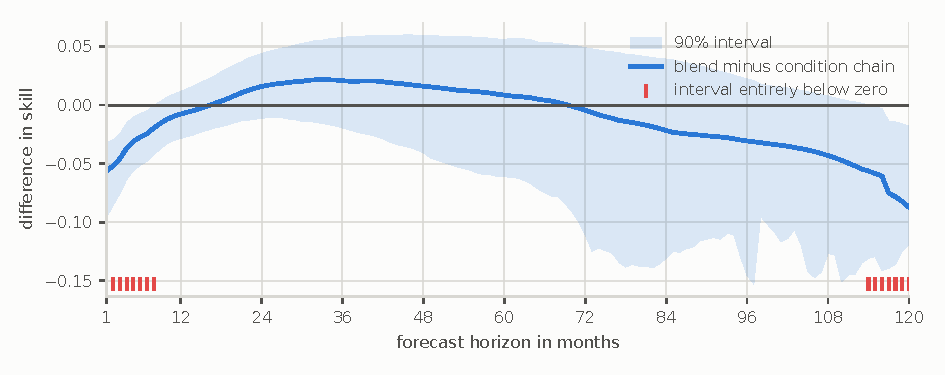
\includegraphics[width=\linewidth]{blend_minus_chain.pdf}
\caption{The blend's skill minus the condition chain's, against R1, with its 90\% interval. Red ticks
mark horizons at which the whole interval lies below zero.}
\label{fig:gap}
\end{figure}

Where the regimes do help is visible question by question (Figure~\ref{fig:by-question}, with the
numbers in Table~\ref{tab:by-question} of Appendix~\ref{app:metrics}). The regime model wins on the questions whose series it observes: inflation
above 5\% and above 3\%, and the federal funds rate falling below 1\%, which the bill rate tracks
closely. It loses where the question is about something it never observes (unemployment and recessions)
and on the \emph{at the horizon} questions, whose answer is mostly whether the condition holds now, which
the regime model's projection ignores. Averaged over the one-year forecasts, the \emph{any time}
questions carry most of the regime model's skill: $+0.302$ against $+0.055$ for the \emph{at the
horizon} questions.


\begin{figure}[t]
\centering
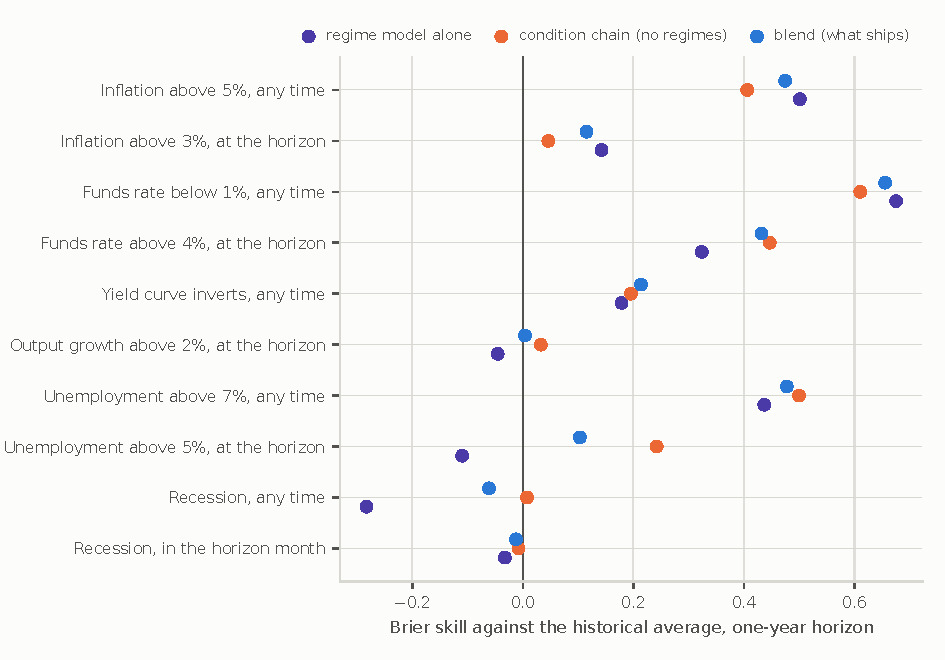
\includegraphics[width=\linewidth]{skill_by_question.pdf}
\caption{One-year skill against R1 for each question and forecaster; the numbers are in
Table~\ref{tab:by-question}. Questions run from those about series the model observes (inflation, the
funds rate through the bill rate, output growth) to unemployment and recessions, which it never
observes.}
\label{fig:by-question}
\end{figure}

\subsection{What improved the forecasts}\label{sec:experiments}

Table~\ref{tab:experiments} summarises the pre-registered experiments; Appendix~\ref{app:experiments}
gives each in full.

\begin{table}[t]
\centering
\caption{Pre-registered experiments: one-year paired difference in mean skill against each experiment's
reference, with intervals at the experiment's family-wise level. A2 and A4 are arms of experiment 0002
(98.33\%); B1 to B3 are arms of experiment 0008 (96.67\%, against R1); experiment 0006 is a single
comparison (90\%). Experiment 0004's row gives the two further seeds' differences.}
\label{tab:experiments}
\small
\begin{tabularx}{\linewidth}{@{}lXrll@{}}
\toprule
Arm & Change & One year & Interval & Reading \\
\midrule
A4 & Two chains (growth; inflation with rates) instead of one & $+0.0590$ & [$+0.0147$, $+0.1019$] & adopted \\
A2 & Four regimes started from growth-by-inflation quadrants & $+0.0381$ & [$+0.0054$, $+0.0690$] & confirmed \\
0004 & A4 re-run with two further seeds & $+0.0603$ & $+0.0603$ & reproduced \\
0006 & Two chains at the single chain's six cells (3$\times$2) & $+0.0587$ & [$+0.0216$, $+0.0934$] & structure helps \\
B1 & At-the-horizon questions through a regime-by-condition chain & $+0.0535$ & [$+0.0174$, $+0.0940$] & miscalibrated \\
B2 & Observe unemployment and the term spread & $-0.0088$ & [$-0.0515$, $+0.0340$] & harmful \\
B3 & Equal blend with the condition chain & $+0.0615$ & [$+0.0341$, $+0.0961$] & adopted \\
\bottomrule
\end{tabularx}
\end{table}

Two changes were adopted. The first replaced one regime chain with two (experiment 0002, arm A4). Of six
pre-registered ideas it had the largest one-year gain over the single chain, cleared the family-wise
bar, passed an independent look-ahead review, and reproduced under two further seeds fixed before they
ran. A later experiment (0006) showed that the gain comes from the two-chain structure rather than from
having more regimes: at the single chain's six cells, two chains still gained $+0.0587$, and a six-cell
two-chain model matches the sixteen-cell one at one year on 27 free parameters against 58.

The second adopted change is the blend (experiment 0008, arm B3), after the condition chain was found to
beat the regime model. Of three pre-registered attempts to close that gap, it gave the largest one-year
gain, $+0.0615$, and it is the only one that passes every gate of rule 0007
at one year. Its rival B1, which runs point-in-time questions through a chain on regime and condition
together, also gained ($+0.0535$) but was overconfident, with calibration slope 0.651. Observing
unemployment and the term spread directly in the regime model (B2) did not help at one year and did harm
at ten ($-0.1176$).

\subsection{Calibration}

Figure~\ref{fig:reliability} compares the regime model's one-year reliability with the blend's. The regime
model is overconfident, with slope \ModelSlopeOneYear{} and interval [0.429, 0.825]: its log-odds need
shrinking by about two fifths. The blend's slope is \BlendSlopeOneYear, and its interval contains one;
the condition chain on its own has slope \ChainSlopeOneYear. Averaging two forecasts pulls probabilities
toward the middle. Here that cures the regime model's overconfidence; averaging forecasts that are each
already calibrated would instead leave the result under-confident \citep{ranjan2010combining}, which is
why the blend's calibration was tested rather than assumed.

\begin{figure}[t]
\centering
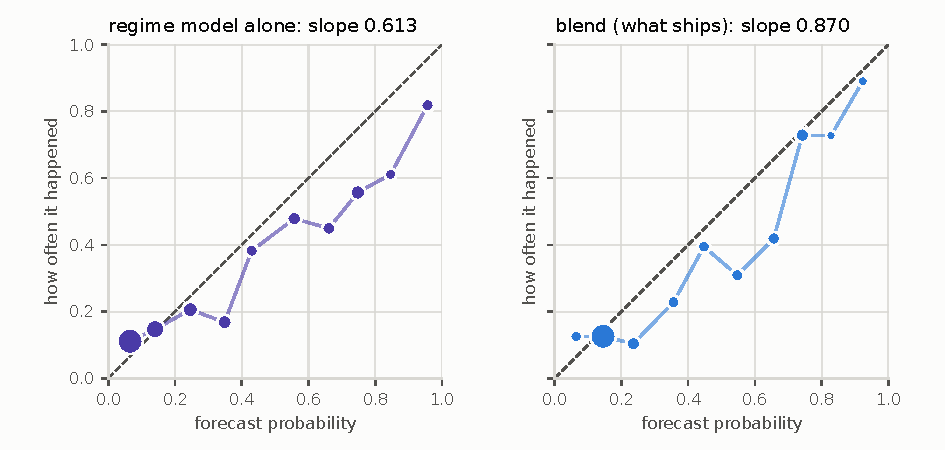
\includegraphics[width=\linewidth]{reliability.pdf}
\caption{Reliability of one-year forecasts, pooled over the ten questions: forecasts are grouped into ten
bins by their probability, and each point shows how often the event happened (vertical axis) against the
average forecast in the bin (horizontal). Point area is the number of forecasts. A calibrated forecaster
lies on the dashed diagonal. The slope is rule 0007's logistic recalibration slope, where one is
calibrated.}
\label{fig:reliability}
\end{figure}

\subsection{What the forecasts see, and what they miss}

Figure~\ref{fig:timelines} shows the one-year forecast that ships through history for four questions,
against the historical average and the months in which the question resolved yes. The forecasts are
most useful in long episodes: once rates reached zero after 2008, or unemployment passed seven percent,
the forecasts stayed high for as long as the episode lasted, while the historical average could not.

\begin{figure}[t]
\centering
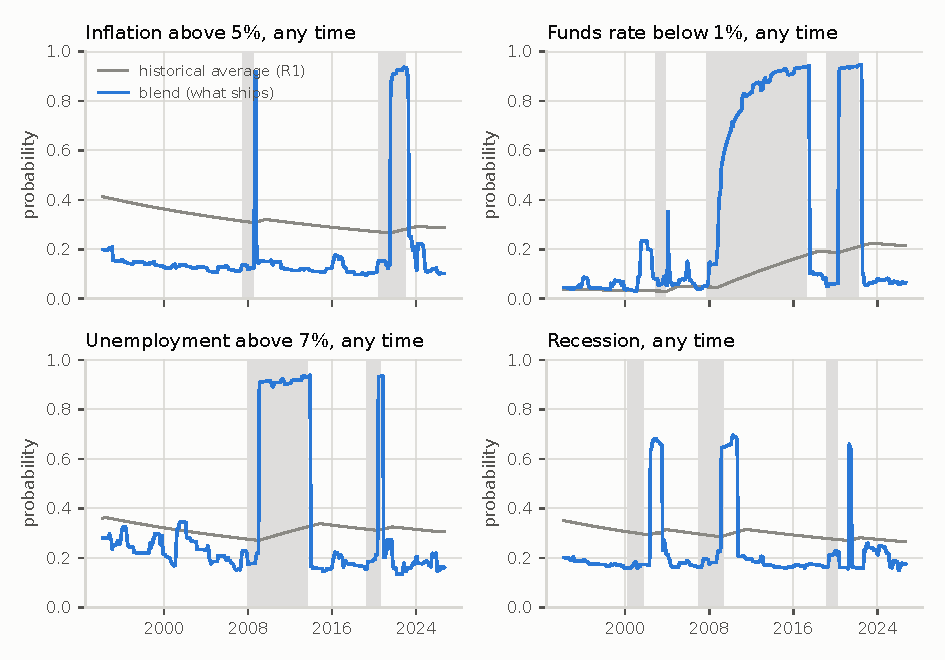
\includegraphics[width=\linewidth]{forecast_timelines.pdf}
\caption{The blend's one-year probability at each forecast date (blue), the historical average R1 (grey),
and, shaded, the forecast dates at which the question resolved yes, meaning the event happened within
the following year.}
\label{fig:timelines}
\end{figure}

They do not anticipate turning points. In July 2021 the blend gave \InflationBeforeSurge{} for inflation
exceeding five percent within a year, below the historical average of \InflationAverageBeforeSurge; a
month later, once readings above five percent had been published, it gave \InflationAfterSurge. The 2001
recession is starker. In April 2001, during the recession, the blend gave \RecessionDuringTwoThousandOne{}
for a recession within a year; in July 2002, after it had ended but before its end was announced, it
gave \RecessionAfterTwoThousandOne. Because recession status is published so late, knowing ``where the
economy is now'' means knowing where it was more than a year ago, and persistence then works against the
forecaster. This is why no forecaster here has meaningful skill on the recession questions.

Figure~\ref{fig:regimes} shows what the two regime chains inferred in real time. The growth chain's
weakest state lights up during and just after the recessions of 2001, 2008--09 and 2020, and in the
industrial slowdown of 2015--16. The levels chain spent most of 1995 to 2021 in its lowest-inflation state; through most of
2022, with inflation high but the bill rate still low, it stayed there, and it moved to its
highest-inflation state only in October 2022, after rates had risen. Because the levels chain reads
inflation and rates together, it recognised the 2021--22 inflation episode late. The blend's inflation
forecasts rose in 2021 through the condition chain half and through the regime model's any-time
composition, which starts from the current condition, not through a change of regime.

\begin{figure}[t]
\centering
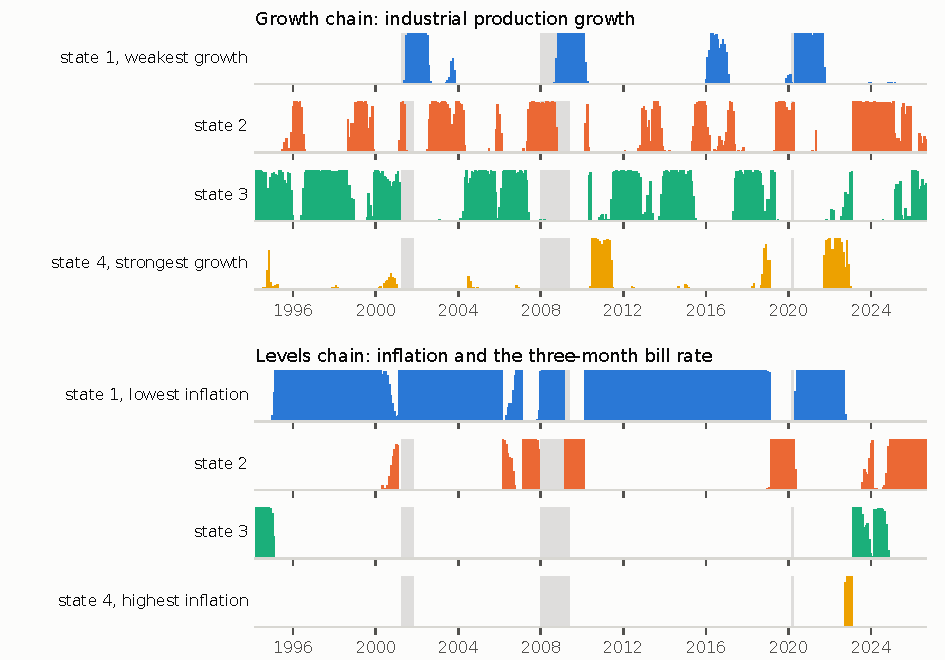
\includegraphics[width=\linewidth]{regime_chains.pdf}
\caption{Filtered probability of each state of the two regime chains at every forecast date, as the model
saw it in real time. States are ordered by their mean growth (growth chain) or mean inflation (levels
chain) at every refit, so a state's rank is comparable across refits while its meaning in natural units
drifts as the sample grows; Appendix~\ref{app:regimes} gives the most recent fit's regimes in natural
units. Shaded bands are NBER recessions.}
\label{fig:regimes}
\end{figure}

\subsection{How honesty changed the answer}\label{sec:honesty}

The headline number did not arrive in a straight line. Table~\ref{tab:history} records how the one-year
verdict changed as problems were found and fixed. No threshold of rule 0001 was moved at any step.

\begin{table}[t]
\centering
\caption{How the one-year result changed. Skill is the mean Brier skill across the ten questions against
the benchmark named. Series start: the average of every outcome since each series began; R1: the average
over the model's own sample.}
\label{tab:history}
\small
\begin{tabularx}{\linewidth}{@{}lXrlp{0.22\linewidth}@{}}
\toprule
2026 & What changed & Skill & Against & One-year verdict \\
\midrule
8 Sep & Rule 0001 committed; first run: one chain, five regimes, forecasts from December 1971 & $+0.232$ & series start & ship the model \\
9 Sep & Two look-ahead paths closed: the number of regimes had been chosen on today's data, and 41\% of forecast dates were fitted on revised prices & $+0.2128$ & series start & ship the average (fails calibration) \\
15 Sep & The benchmark had counted outcomes before they were published; fixed & $+0.2154$ & series start & ship the average \\
20 Sep & Two chains adopted (experiment 0002, arm A4) & $+0.2744$ & series start & ship the model \\
21 Sep & Recession months dated by their announcement & $+0.2673$ & series start & ship the model \\
29 Sep & Fair benchmark R1; the condition chain beats the model & $+0.1786$ & R1 & ship the average under 0007 (fails calibration and the chain) \\
29 Sep & Blend adopted (experiment 0008, arm B3) & $+0.2401$ & R1 & ship the model under both rules \\
\bottomrule
\end{tabularx}
\end{table}

Two lessons stand out. The first run's one-year verdict matched its prediction but did not survive: two
look-ahead paths had to be closed, and with either one closed the one-year verdict was lost. The more
instructive leak was found by execution rather than by reading. The audit of Section~\ref{sec:audit},
run for the first time, showed that 12 of 2,190 forecasts issued up to its cutoff changed when only
unavailable information was perturbed, and every one of them was the benchmark: at each date it had
counted outcomes resting on values not yet published, by 400 days for recession dating. A unit test had
pinned the faulty behaviour as the specification, so code and test agreed with each other. Later, the
first attempt to date recessions by their announcements leaked worse than the problem it fixed; the
same audit caught it with more than 400 changed forecasts before it was merged.

The second lesson is about benchmarks. Moving from the average since each series began to the average
over the model's own sample lowered the regime model's one-year skill from $+0.2673$ to $+0.1786$. That
was not a leak, but its effect on the reported skill was that of a weak benchmark, and it was largest
for the recession questions, whose average reached back to 1854.

\subsection{What ships}

Table~\ref{tab:shipped} in Appendix~\ref{app:shipped} gives the forecasts released with this paper,
from data as of 1 August 2026. At
one year they are the blend, shown with both halves; at five and ten years they are R1. They are
registered forward, together with the regime model alone, the single-chain model, the condition chain
and R1 as companions, and will be scored as they resolve. The first one-year claims resolve on 1 July
2027.


\section{Discussion}\label{sec:discussion}

\paragraph{What this means for a reader who wants a forecast.} One year ahead, a probability that knows
where the economy is now, adjusted by what the regimes know about inflation and interest rates, is
clearly better than the historical average. Four years ahead it is not, and a forecaster who quotes a
precise five- or ten-year probability for these questions claims more than thirty years of evidence can
support. Recessions remain the hardest case: they are dated so late that even knowing the present is
impossible in real time.

\paragraph{What this means for forecasters.} Three habits changed our conclusions and would change
others'. Always report skill against persistence as well as against the average, because a skill score
against the average alone mixes the value of knowing the present with the value of the model. Check where
the benchmark's window starts, because an average that reaches further back than the model's data can
flatter every score. And audit look-ahead by execution: perturb what a forecast should not know and
require it not to move, because a leak can live in the benchmark rather than the model, and code and its
tests can agree on the wrong specification.

\paragraph{Limitations.}
\begin{itemize}[leftmargin=*]
\item \emph{Everything here is in sample.} The two adopted changes were designed after this sample's
  results had been seen. \textsc{Confirmed in sample} is the ceiling of what the backtest can say; the
  forward register is the only out-of-sample test, and matching the backtest's power that way will take
  decades.
\item \emph{One sample, few independent observations.} About 31 at one year and 5.5 at five years. The
  one-month location of any horizon (46 rather than 45 or 48) is not meaningful.
\item \emph{The walk-forward starts in 1994.} No forecast is scored during the 1970s inflation, although
  the model learns from it.
\item \emph{Two small known departures from real time.} The conditions from which the rates are learned are read from final
  data with publication timing enforced; for output growth this differs from the published vintage in
  0.987\% of condition-months (0.084\% for inflation above three percent). And on 11 of the 391
  forecast dates, where the condition chain starts for the recession questions depended on a turning
  point announced after the forecast date. Their measured effects at one year are $+0.0007$ and
  $-0.0007$, below the registered floor of 0.001. Independent reviews found both, today's forecasts are
  unaffected by the second, and both are scheduled for correction.
\item \emph{Four by four is at the top of its range.} Each chain was offered at most four states and both
  took four; the range may be binding.
\item \emph{The calibration test is imperfect.} Its intervals under-cover on outcomes this persistent,
  and it fails a perfectly calibrated forecaster about one time in four.
\item \emph{Rule 0007 and the adoption of the blend were delegated decisions}
  (Section~\ref{sec:delegation}), and rule 0007 was written after the numbers that motivated it were
  known.
\end{itemize}

\paragraph{Next steps.} Already scheduled: correcting the two approximations above; testing the smaller
six-cell model under the blend (experiment 0011); extending the consumer price series back to 1972 with
the unrevised index, which would bring the 1970s into the scored sample (experiment 0009); and continuing
the monthly forward register.

\section{Conclusion}\label{sec:conclusion}

We asked how far ahead probability forecasts of ten US macroeconomic events can beat the historical
average when they are built only from data published by each forecast date and judged by rules fixed in
advance.
The answer is about two and a half years for a regime model and about four years for a blend of that
model with a forecaster that knows only where each condition stands now. Most of the one-year skill
comes from persistence, and regimes add information mainly about inflation and interest rates. Beyond
about four years we ship the historical average, and we say so. Getting to that answer required finding
and fixing leaks that had made the method look better than it was, and choosing a benchmark as strong as
it honestly could be. The forecasts are now registered forward, and the future will score them.

\section*{Data and code availability}

All data are public and are fetched without an API key from FRED and ALFRED
\citep{stlouisfed2026fred,stlouisfed2026alfred} and from the NBER's business cycle pages
\citep{nber2026cycles,nber2026announcements}. The code, the registries of series and questions, every
pre-registration and experiment record, the committed baselines behind every table, and the forward
register are in the repository named on the first page. Every table and figure in this paper is
regenerated from committed records by \texttt{forecast paper-assets}, and a test requires every other
number in the text to appear in a committed record.

\section*{Reproducibility}

Runs are deterministic: seeds are fixed, every result row carries a configuration hash, and two runs of
the same configuration produce byte-identical outputs. The configuration reported here is
\texttt{7647c129be85291e}; the regime model alone is \texttt{fec79a040f9ca6f9}. The five acceptance
gates, the look-ahead audit at both cutoffs and the test suite all pass on the commit that builds this
paper.

\section*{Use of AI tools}

The software, the analyses and the drafting of this paper were carried out with extensive assistance
from AI coding agents (Anthropic's Claude models, operated through Claude Code). On 29 September 2026
research decisions were delegated to one such model, as described in Section~\ref{sec:delegation}; those
decisions are recorded verbatim and labelled as delegated. The references were checked against their
publishers' records. The author is responsible for the content.

\section*{Competing interests and funding}

% CONFIRM with the author before submission.
The author declares no competing interests. This work received no external funding.

\bibliographystyle{plainnat}
\bibliography{references}

\clearpage
\appendix

\section{Glossary}\label{app:glossary}

\begin{description}[leftmargin=0pt,style=nextline]
\item[Any time / at the horizon] Two kinds of question: whether a condition holds in at least one month
  up to the horizon, or in the horizon month alone.
\item[Blend] The forecast that ships: half the regime model plus half the condition chain.
\item[Brier score] Mean squared difference between forecast probabilities and outcomes (one or zero).
  Lower is better.
\item[Brier skill score] One minus the forecaster's Brier score divided by a reference's. Positive
  beats the reference.
\item[Calibration] Whether events forecast at $p$ happen about a fraction $p$ of the time.
\item[Condition chain (R2)] A two-state Markov chain on a question's own monthly condition, with an entry
  hazard and a persistence, and no regimes.
\item[Effective independent observations] Resolved forecast dates divided by the bootstrap block length;
  how many truly separate pieces of evidence overlapping forecasts amount to.
\item[Filtered probability] The probability of a regime given data up to that month only. Smoothed
  probabilities, which use later data, are never used in the backtest.
\item[Historical average (R1)] The fraction of past outcomes that resolved yes, counting only outcomes
  published by the forecast date and inside the model's own sample.
\item[Look-ahead] Any use of information that was not available on the forecast date.
\item[Moving-block bootstrap] Resampling whole blocks of consecutive forecast dates to measure
  uncertainty while keeping their dependence.
\item[NBER] The National Bureau of Economic Research, whose committee dates US recessions.
\item[Pre-registration] Committing hypotheses, thresholds and the decision rule before seeing results.
\item[Regime] A persistent state of the economy with its own typical growth, inflation and rates.
\item[Ship-the-average horizon] The last horizon up to which a forecaster beats the historical average
  without a break.
\item[Vintage] The version of a data series as it was published on a given date, before later revisions.
\end{description}

\section{The decision rules in full}\label{app:rules}

Both rules are files that the pipeline reads and applies:
\begin{itemize}[leftmargin=*]
\item rule 0001: \path{proving/experiments/0001-regime-conditional-forecast-skill/experiment.json};
\item rule 0007: \path{proving/experiments/0007-successor-evaluation-rule/experiment.json}.
\end{itemize}
Table~\ref{tab:gates} summarises their gates. The rules share their
thresholds, bootstrap settings (moving blocks of at least the horizon, 10,000 resamples, seed 20260908)
and failure action (ship the average for that horizon and record the failing gate). They differ in the
benchmark (the average since each series began, against R1), the calibration test (ten-bin error below
0.10, against the logistic slope test), and in the last gate (whether regimes exist, against whether the
condition chain beats the model). Rule 0007 also requires the pooled skill, one minus the ratio of
summed Brier scores, to agree in sign with the mean of per-question skills. Its registration records two
dated clarifications made after experiment 0008's arms had run; neither moved a threshold.

\section{Skill at every horizon}\label{app:every-month}

{\footnotesize
\setlength{\tabcolsep}{3pt}
\begin{longtable}{rllllr}
\caption{Brier skill against the historical average (R1) at every horizon, with 90\% moving-block bootstrap intervals. \emph{Indep.} is the number of effectively independent observations behind each estimate. Source: measurement 0010, \texttt{research/reports/skill-at-every-horizon/}.}\label{tab:every-month}\\
\toprule
Months & Regime model alone & Blend & Condition chain & Blend $-$ chain & Indep. \\
\midrule
\endfirsthead
\toprule
Months & Regime model alone & Blend & Condition chain & Blend $-$ chain & Indep. \\
\midrule
\endhead
\midrule
\multicolumn{6}{r}{\footnotesize continued on the next page}\\
\endfoot
\bottomrule
\endlastfoot
1 & $+0.290$ {\scriptsize [$+0.161$, $+0.369$]} & $+0.476$ {\scriptsize [$+0.406$, $+0.531$]} & $+0.532$ {\scriptsize [$+0.477$, $+0.580$]} & $-0.056$ {\scriptsize [$-0.096$, $-0.033$]} & 32.4 \\
2 & $+0.278$ {\scriptsize [$+0.170$, $+0.354$]} & $+0.443$ {\scriptsize [$+0.377$, $+0.501$]} & $+0.495$ {\scriptsize [$+0.437$, $+0.546$]} & $-0.052$ {\scriptsize [$-0.086$, $-0.030$]} & 32.3 \\
3 & $+0.268$ {\scriptsize [$+0.175$, $+0.344$]} & $+0.414$ {\scriptsize [$+0.350$, $+0.475$]} & $+0.460$ {\scriptsize [$+0.400$, $+0.515$]} & $-0.046$ {\scriptsize [$-0.076$, $-0.024$]} & 32.2 \\
4 & $+0.260$ {\scriptsize [$+0.174$, $+0.333$]} & $+0.387$ {\scriptsize [$+0.322$, $+0.449$]} & $+0.423$ {\scriptsize [$+0.360$, $+0.480$]} & $-0.037$ {\scriptsize [$-0.064$, $-0.015$]} & 32.2 \\
5 & $+0.249$ {\scriptsize [$+0.167$, $+0.323$]} & $+0.362$ {\scriptsize [$+0.297$, $+0.426$]} & $+0.393$ {\scriptsize [$+0.328$, $+0.452$]} & $-0.031$ {\scriptsize [$-0.056$, $-0.010$]} & 32.1 \\
6 & $+0.236$ {\scriptsize [$+0.155$, $+0.312$]} & $+0.339$ {\scriptsize [$+0.272$, $+0.405$]} & $+0.367$ {\scriptsize [$+0.300$, $+0.427$]} & $-0.027$ {\scriptsize [$-0.052$, $-0.007$]} & 32.0 \\
7 & $+0.224$ {\scriptsize [$+0.144$, $+0.300$]} & $+0.318$ {\scriptsize [$+0.251$, $+0.386$]} & $+0.343$ {\scriptsize [$+0.277$, $+0.405$]} & $-0.025$ {\scriptsize [$-0.048$, $-0.005$]} & 31.9 \\
8 & $+0.212$ {\scriptsize [$+0.134$, $+0.289$]} & $+0.298$ {\scriptsize [$+0.230$, $+0.366$]} & $+0.317$ {\scriptsize [$+0.251$, $+0.381$]} & $-0.020$ {\scriptsize [$-0.043$, $-0.001$]} & 31.8 \\
9 & $+0.204$ {\scriptsize [$+0.126$, $+0.282$]} & $+0.281$ {\scriptsize [$+0.213$, $+0.351$]} & $+0.297$ {\scriptsize [$+0.230$, $+0.362$]} & $-0.016$ {\scriptsize [$-0.037$, $+0.003$]} & 31.8 \\
10 & $+0.195$ {\scriptsize [$+0.119$, $+0.273$]} & $+0.266$ {\scriptsize [$+0.197$, $+0.336$]} & $+0.278$ {\scriptsize [$+0.211$, $+0.343$]} & $-0.012$ {\scriptsize [$-0.033$, $+0.007$]} & 31.7 \\
11 & $+0.186$ {\scriptsize [$+0.109$, $+0.265$]} & $+0.252$ {\scriptsize [$+0.183$, $+0.323$]} & $+0.262$ {\scriptsize [$+0.196$, $+0.327$]} & $-0.010$ {\scriptsize [$-0.030$, $+0.009$]} & 31.6 \\
12 & $+0.179$ {\scriptsize [$+0.102$, $+0.258$]} & $+0.240$ {\scriptsize [$+0.172$, $+0.311$]} & $+0.248$ {\scriptsize [$+0.183$, $+0.312$]} & $-0.008$ {\scriptsize [$-0.028$, $+0.012$]} & 31.5 \\
13 & $+0.171$ {\scriptsize [$+0.093$, $+0.253$]} & $+0.229$ {\scriptsize [$+0.159$, $+0.302$]} & $+0.235$ {\scriptsize [$+0.169$, $+0.301$]} & $-0.006$ {\scriptsize [$-0.027$, $+0.014$]} & 29.0 \\
14 & $+0.164$ {\scriptsize [$+0.084$, $+0.248$]} & $+0.219$ {\scriptsize [$+0.148$, $+0.293$]} & $+0.224$ {\scriptsize [$+0.156$, $+0.289$]} & $-0.005$ {\scriptsize [$-0.025$, $+0.016$]} & 26.9 \\
15 & $+0.158$ {\scriptsize [$+0.075$, $+0.245$]} & $+0.209$ {\scriptsize [$+0.136$, $+0.285$]} & $+0.212$ {\scriptsize [$+0.144$, $+0.278$]} & $-0.003$ {\scriptsize [$-0.023$, $+0.019$]} & 25.0 \\
16 & $+0.153$ {\scriptsize [$+0.069$, $+0.241$]} & $+0.201$ {\scriptsize [$+0.127$, $+0.277$]} & $+0.202$ {\scriptsize [$+0.134$, $+0.267$]} & $-0.001$ {\scriptsize [$-0.022$, $+0.022$]} & 23.4 \\
17 & $+0.149$ {\scriptsize [$+0.063$, $+0.239$]} & $+0.194$ {\scriptsize [$+0.118$, $+0.271$]} & $+0.193$ {\scriptsize [$+0.123$, $+0.257$]} & $+0.001$ {\scriptsize [$-0.020$, $+0.025$]} & 21.9 \\
18 & $+0.146$ {\scriptsize [$+0.058$, $+0.237$]} & $+0.188$ {\scriptsize [$+0.112$, $+0.264$]} & $+0.185$ {\scriptsize [$+0.117$, $+0.247$]} & $+0.003$ {\scriptsize [$-0.018$, $+0.028$]} & 20.7 \\
19 & $+0.143$ {\scriptsize [$+0.050$, $+0.235$]} & $+0.182$ {\scriptsize [$+0.102$, $+0.258$]} & $+0.176$ {\scriptsize [$+0.108$, $+0.237$]} & $+0.006$ {\scriptsize [$-0.017$, $+0.031$]} & 19.5 \\
20 & $+0.141$ {\scriptsize [$+0.047$, $+0.236$]} & $+0.177$ {\scriptsize [$+0.097$, $+0.253$]} & $+0.169$ {\scriptsize [$+0.099$, $+0.228$]} & $+0.008$ {\scriptsize [$-0.015$, $+0.034$]} & 18.5 \\
21 & $+0.140$ {\scriptsize [$+0.042$, $+0.232$]} & $+0.172$ {\scriptsize [$+0.089$, $+0.246$]} & $+0.162$ {\scriptsize [$+0.092$, $+0.219$]} & $+0.010$ {\scriptsize [$-0.014$, $+0.037$]} & 17.6 \\
22 & $+0.139$ {\scriptsize [$+0.036$, $+0.233$]} & $+0.168$ {\scriptsize [$+0.082$, $+0.242$]} & $+0.156$ {\scriptsize [$+0.085$, $+0.212$]} & $+0.013$ {\scriptsize [$-0.013$, $+0.040$]} & 16.7 \\
23 & $+0.137$ {\scriptsize [$+0.031$, $+0.232$]} & $+0.164$ {\scriptsize [$+0.077$, $+0.240$]} & $+0.150$ {\scriptsize [$+0.079$, $+0.206$]} & $+0.014$ {\scriptsize [$-0.012$, $+0.042$]} & 16.0 \\
24 & $+0.135$ {\scriptsize [$+0.027$, $+0.231$]} & $+0.160$ {\scriptsize [$+0.072$, $+0.235$]} & $+0.144$ {\scriptsize [$+0.073$, $+0.201$]} & $+0.016$ {\scriptsize [$-0.011$, $+0.044$]} & 15.2 \\
25 & $+0.133$ {\scriptsize [$+0.024$, $+0.231$]} & $+0.156$ {\scriptsize [$+0.068$, $+0.233$]} & $+0.139$ {\scriptsize [$+0.070$, $+0.196$]} & $+0.017$ {\scriptsize [$-0.011$, $+0.046$]} & 14.6 \\
26 & $+0.131$ {\scriptsize [$+0.018$, $+0.228$]} & $+0.152$ {\scriptsize [$+0.062$, $+0.229$]} & $+0.134$ {\scriptsize [$+0.066$, $+0.191$]} & $+0.018$ {\scriptsize [$-0.011$, $+0.047$]} & 14.0 \\
27 & $+0.128$ {\scriptsize [$+0.014$, $+0.227$]} & $+0.149$ {\scriptsize [$+0.059$, $+0.224$]} & $+0.130$ {\scriptsize [$+0.063$, $+0.185$]} & $+0.019$ {\scriptsize [$-0.011$, $+0.049$]} & 13.4 \\
28 & $+0.125$ {\scriptsize [$+0.008$, $+0.227$]} & $+0.145$ {\scriptsize [$+0.053$, $+0.223$]} & $+0.126$ {\scriptsize [$+0.058$, $+0.180$]} & $+0.019$ {\scriptsize [$-0.012$, $+0.050$]} & 12.9 \\
29 & $+0.123$ {\scriptsize [$+0.005$, $+0.225$]} & $+0.141$ {\scriptsize [$+0.050$, $+0.219$]} & $+0.122$ {\scriptsize [$+0.056$, $+0.175$]} & $+0.020$ {\scriptsize [$-0.012$, $+0.051$]} & 12.4 \\
30 & $+0.121$ {\scriptsize [$-0.002$, $+0.225$]} & $+0.139$ {\scriptsize [$+0.046$, $+0.218$]} & $+0.119$ {\scriptsize [$+0.052$, $+0.172$]} & $+0.020$ {\scriptsize [$-0.014$, $+0.053$]} & 12.0 \\
31 & $+0.121$ {\scriptsize [$-0.003$, $+0.226$]} & $+0.138$ {\scriptsize [$+0.044$, $+0.216$]} & $+0.117$ {\scriptsize [$+0.052$, $+0.169$]} & $+0.021$ {\scriptsize [$-0.014$, $+0.054$]} & 11.6 \\
32 & $+0.121$ {\scriptsize [$-0.007$, $+0.226$]} & $+0.137$ {\scriptsize [$+0.042$, $+0.215$]} & $+0.116$ {\scriptsize [$+0.050$, $+0.167$]} & $+0.022$ {\scriptsize [$-0.015$, $+0.055$]} & 11.2 \\
33 & $+0.118$ {\scriptsize [$-0.012$, $+0.222$]} & $+0.134$ {\scriptsize [$+0.038$, $+0.210$]} & $+0.112$ {\scriptsize [$+0.047$, $+0.163$]} & $+0.022$ {\scriptsize [$-0.016$, $+0.055$]} & 10.8 \\
34 & $+0.116$ {\scriptsize [$-0.014$, $+0.221$]} & $+0.132$ {\scriptsize [$+0.036$, $+0.209$]} & $+0.110$ {\scriptsize [$+0.046$, $+0.160$]} & $+0.022$ {\scriptsize [$-0.017$, $+0.057$]} & 10.5 \\
35 & $+0.113$ {\scriptsize [$-0.019$, $+0.220$]} & $+0.129$ {\scriptsize [$+0.032$, $+0.205$]} & $+0.108$ {\scriptsize [$+0.043$, $+0.156$]} & $+0.021$ {\scriptsize [$-0.018$, $+0.057$]} & 10.1 \\
36 & $+0.109$ {\scriptsize [$-0.025$, $+0.216$]} & $+0.126$ {\scriptsize [$+0.029$, $+0.202$]} & $+0.105$ {\scriptsize [$+0.041$, $+0.152$]} & $+0.021$ {\scriptsize [$-0.019$, $+0.058$]} & 9.8 \\
37 & $+0.106$ {\scriptsize [$-0.030$, $+0.216$]} & $+0.123$ {\scriptsize [$+0.026$, $+0.200$]} & $+0.103$ {\scriptsize [$+0.040$, $+0.149$]} & $+0.020$ {\scriptsize [$-0.021$, $+0.058$]} & 9.5 \\
38 & $+0.104$ {\scriptsize [$-0.035$, $+0.214$]} & $+0.121$ {\scriptsize [$+0.023$, $+0.197$]} & $+0.100$ {\scriptsize [$+0.038$, $+0.147$]} & $+0.020$ {\scriptsize [$-0.023$, $+0.059$]} & 9.3 \\
39 & $+0.102$ {\scriptsize [$-0.042$, $+0.214$]} & $+0.118$ {\scriptsize [$+0.019$, $+0.196$]} & $+0.098$ {\scriptsize [$+0.035$, $+0.144$]} & $+0.020$ {\scriptsize [$-0.024$, $+0.059$]} & 9.0 \\
40 & $+0.100$ {\scriptsize [$-0.045$, $+0.211$]} & $+0.116$ {\scriptsize [$+0.016$, $+0.193$]} & $+0.096$ {\scriptsize [$+0.034$, $+0.141$]} & $+0.021$ {\scriptsize [$-0.025$, $+0.059$]} & 8.8 \\
41 & $+0.097$ {\scriptsize [$-0.049$, $+0.209$]} & $+0.113$ {\scriptsize [$+0.013$, $+0.189$]} & $+0.093$ {\scriptsize [$+0.032$, $+0.138$]} & $+0.020$ {\scriptsize [$-0.027$, $+0.060$]} & 8.5 \\
42 & $+0.093$ {\scriptsize [$-0.054$, $+0.206$]} & $+0.110$ {\scriptsize [$+0.010$, $+0.187$]} & $+0.091$ {\scriptsize [$+0.031$, $+0.135$]} & $+0.020$ {\scriptsize [$-0.029$, $+0.060$]} & 8.3 \\
43 & $+0.090$ {\scriptsize [$-0.060$, $+0.206$]} & $+0.108$ {\scriptsize [$+0.006$, $+0.185$]} & $+0.089$ {\scriptsize [$+0.030$, $+0.133$]} & $+0.019$ {\scriptsize [$-0.031$, $+0.060$]} & 8.1 \\
44 & $+0.088$ {\scriptsize [$-0.065$, $+0.204$]} & $+0.106$ {\scriptsize [$+0.004$, $+0.184$]} & $+0.087$ {\scriptsize [$+0.029$, $+0.132$]} & $+0.019$ {\scriptsize [$-0.034$, $+0.060$]} & 7.9 \\
45 & $+0.085$ {\scriptsize [$-0.069$, $+0.203$]} & $+0.104$ {\scriptsize [$+0.002$, $+0.184$]} & $+0.086$ {\scriptsize [$+0.028$, $+0.130$]} & $+0.018$ {\scriptsize [$-0.035$, $+0.060$]} & 7.7 \\
46 & $+0.083$ {\scriptsize [$-0.073$, $+0.202$]} & $+0.102$ {\scriptsize [$+0.000$, $+0.182$]} & $+0.085$ {\scriptsize [$+0.028$, $+0.129$]} & $+0.017$ {\scriptsize [$-0.036$, $+0.060$]} & 7.5 \\
47 & $+0.080$ {\scriptsize [$-0.079$, $+0.202$]} & $+0.100$ {\scriptsize [$-0.002$, $+0.181$]} & $+0.084$ {\scriptsize [$+0.029$, $+0.127$]} & $+0.017$ {\scriptsize [$-0.038$, $+0.060$]} & 7.3 \\
48 & $+0.078$ {\scriptsize [$-0.085$, $+0.201$]} & $+0.099$ {\scriptsize [$-0.005$, $+0.180$]} & $+0.083$ {\scriptsize [$+0.029$, $+0.126$]} & $+0.016$ {\scriptsize [$-0.041$, $+0.060$]} & 7.1 \\
49 & $+0.077$ {\scriptsize [$-0.093$, $+0.197$]} & $+0.098$ {\scriptsize [$-0.009$, $+0.177$]} & $+0.082$ {\scriptsize [$+0.028$, $+0.124$]} & $+0.016$ {\scriptsize [$-0.045$, $+0.059$]} & 7.0 \\
50 & $+0.075$ {\scriptsize [$-0.098$, $+0.196$]} & $+0.097$ {\scriptsize [$-0.011$, $+0.176$]} & $+0.082$ {\scriptsize [$+0.029$, $+0.123$]} & $+0.015$ {\scriptsize [$-0.047$, $+0.059$]} & 6.8 \\
51 & $+0.074$ {\scriptsize [$-0.102$, $+0.195$]} & $+0.096$ {\scriptsize [$-0.012$, $+0.174$]} & $+0.082$ {\scriptsize [$+0.029$, $+0.122$]} & $+0.014$ {\scriptsize [$-0.049$, $+0.058$]} & 6.6 \\
52 & $+0.073$ {\scriptsize [$-0.103$, $+0.195$]} & $+0.096$ {\scriptsize [$-0.012$, $+0.172$]} & $+0.082$ {\scriptsize [$+0.030$, $+0.121$]} & $+0.014$ {\scriptsize [$-0.051$, $+0.059$]} & 6.5 \\
53 & $+0.071$ {\scriptsize [$-0.108$, $+0.194$]} & $+0.095$ {\scriptsize [$-0.013$, $+0.173$]} & $+0.082$ {\scriptsize [$+0.032$, $+0.120$]} & $+0.013$ {\scriptsize [$-0.053$, $+0.058$]} & 6.4 \\
54 & $+0.071$ {\scriptsize [$-0.109$, $+0.194$]} & $+0.095$ {\scriptsize [$-0.013$, $+0.173$]} & $+0.083$ {\scriptsize [$+0.034$, $+0.120$]} & $+0.012$ {\scriptsize [$-0.054$, $+0.058$]} & 6.2 \\
55 & $+0.071$ {\scriptsize [$-0.114$, $+0.194$]} & $+0.095$ {\scriptsize [$-0.015$, $+0.172$]} & $+0.083$ {\scriptsize [$+0.035$, $+0.120$]} & $+0.012$ {\scriptsize [$-0.056$, $+0.058$]} & 6.1 \\
56 & $+0.071$ {\scriptsize [$-0.117$, $+0.193$]} & $+0.096$ {\scriptsize [$-0.015$, $+0.172$]} & $+0.084$ {\scriptsize [$+0.036$, $+0.120$]} & $+0.011$ {\scriptsize [$-0.058$, $+0.058$]} & 6.0 \\
57 & $+0.070$ {\scriptsize [$-0.120$, $+0.193$]} & $+0.096$ {\scriptsize [$-0.014$, $+0.171$]} & $+0.085$ {\scriptsize [$+0.038$, $+0.121$]} & $+0.011$ {\scriptsize [$-0.059$, $+0.058$]} & 5.8 \\
58 & $+0.069$ {\scriptsize [$-0.121$, $+0.189$]} & $+0.096$ {\scriptsize [$-0.015$, $+0.169$]} & $+0.086$ {\scriptsize [$+0.038$, $+0.118$]} & $+0.010$ {\scriptsize [$-0.059$, $+0.057$]} & 5.7 \\
59 & $+0.069$ {\scriptsize [$-0.122$, $+0.189$]} & $+0.096$ {\scriptsize [$-0.013$, $+0.169$]} & $+0.087$ {\scriptsize [$+0.039$, $+0.119$]} & $+0.009$ {\scriptsize [$-0.061$, $+0.056$]} & 5.6 \\
60 & $+0.069$ {\scriptsize [$-0.121$, $+0.191$]} & $+0.097$ {\scriptsize [$-0.012$, $+0.169$]} & $+0.088$ {\scriptsize [$+0.042$, $+0.119$]} & $+0.008$ {\scriptsize [$-0.061$, $+0.056$]} & 5.5 \\
61 & $+0.069$ {\scriptsize [$-0.120$, $+0.192$]} & $+0.098$ {\scriptsize [$-0.010$, $+0.169$]} & $+0.090$ {\scriptsize [$+0.045$, $+0.119$]} & $+0.008$ {\scriptsize [$-0.062$, $+0.056$]} & 5.4 \\
62 & $+0.069$ {\scriptsize [$-0.122$, $+0.192$]} & $+0.098$ {\scriptsize [$-0.009$, $+0.170$]} & $+0.091$ {\scriptsize [$+0.047$, $+0.120$]} & $+0.007$ {\scriptsize [$-0.062$, $+0.057$]} & 5.3 \\
63 & $+0.069$ {\scriptsize [$-0.125$, $+0.193$]} & $+0.099$ {\scriptsize [$-0.010$, $+0.170$]} & $+0.092$ {\scriptsize [$+0.048$, $+0.120$]} & $+0.007$ {\scriptsize [$-0.065$, $+0.056$]} & 5.2 \\
64 & $+0.068$ {\scriptsize [$-0.131$, $+0.192$]} & $+0.099$ {\scriptsize [$-0.011$, $+0.170$]} & $+0.093$ {\scriptsize [$+0.049$, $+0.121$]} & $+0.006$ {\scriptsize [$-0.068$, $+0.056$]} & 5.1 \\
65 & $+0.067$ {\scriptsize [$-0.140$, $+0.185$]} & $+0.099$ {\scriptsize [$-0.015$, $+0.167$]} & $+0.094$ {\scriptsize [$+0.050$, $+0.121$]} & $+0.005$ {\scriptsize [$-0.072$, $+0.054$]} & 5.0 \\
66 & $+0.067$ {\scriptsize [$-0.148$, $+0.187$]} & $+0.100$ {\scriptsize [$-0.017$, $+0.168$]} & $+0.096$ {\scriptsize [$+0.051$, $+0.123$]} & $+0.004$ {\scriptsize [$-0.075$, $+0.054$]} & 4.9 \\
67 & $+0.067$ {\scriptsize [$-0.154$, $+0.187$]} & $+0.101$ {\scriptsize [$-0.018$, $+0.169$]} & $+0.097$ {\scriptsize [$+0.052$, $+0.125$]} & $+0.003$ {\scriptsize [$-0.078$, $+0.053$]} & 4.8 \\
68 & $+0.066$ {\scriptsize [$-0.155$, $+0.187$]} & $+0.101$ {\scriptsize [$-0.017$, $+0.169$]} & $+0.099$ {\scriptsize [$+0.054$, $+0.127$]} & $+0.002$ {\scriptsize [$-0.078$, $+0.053$]} & 4.7 \\
69 & $+0.063$ {\scriptsize [$-0.171$, $+0.186$]} & $+0.100$ {\scriptsize [$-0.023$, $+0.168$]} & $+0.099$ {\scriptsize [$+0.053$, $+0.127$]} & $+0.001$ {\scriptsize [$-0.084$, $+0.052$]} & 4.7 \\
70 & $+0.059$ {\scriptsize [$-0.187$, $+0.185$]} & $+0.098$ {\scriptsize [$-0.034$, $+0.167$]} & $+0.099$ {\scriptsize [$+0.052$, $+0.128$]} & $-0.001$ {\scriptsize [$-0.091$, $+0.051$]} & 4.6 \\
71 & $+0.056$ {\scriptsize [$-0.213$, $+0.183$]} & $+0.097$ {\scriptsize [$-0.045$, $+0.167$]} & $+0.099$ {\scriptsize [$+0.049$, $+0.128$]} & $-0.003$ {\scriptsize [$-0.099$, $+0.050$]} & 4.5 \\
72 & $+0.052$ {\scriptsize [$-0.247$, $+0.180$]} & $+0.095$ {\scriptsize [$-0.063$, $+0.165$]} & $+0.099$ {\scriptsize [$+0.044$, $+0.128$]} & $-0.004$ {\scriptsize [$-0.111$, $+0.049$]} & 4.4 \\
73 & $+0.048$ {\scriptsize [$-0.286$, $+0.178$]} & $+0.093$ {\scriptsize [$-0.086$, $+0.163$]} & $+0.099$ {\scriptsize [$+0.036$, $+0.128$]} & $-0.006$ {\scriptsize [$-0.125$, $+0.048$]} & 4.3 \\
74 & $+0.044$ {\scriptsize [$-0.273$, $+0.176$]} & $+0.091$ {\scriptsize [$-0.077$, $+0.161$]} & $+0.099$ {\scriptsize [$+0.040$, $+0.128$]} & $-0.008$ {\scriptsize [$-0.122$, $+0.047$]} & 4.3 \\
75 & $+0.040$ {\scriptsize [$-0.284$, $+0.174$]} & $+0.089$ {\scriptsize [$-0.081$, $+0.160$]} & $+0.099$ {\scriptsize [$+0.040$, $+0.128$]} & $-0.010$ {\scriptsize [$-0.124$, $+0.046$]} & 4.2 \\
76 & $+0.037$ {\scriptsize [$-0.289$, $+0.173$]} & $+0.088$ {\scriptsize [$-0.084$, $+0.161$]} & $+0.100$ {\scriptsize [$+0.040$, $+0.130$]} & $-0.011$ {\scriptsize [$-0.126$, $+0.045$]} & 4.1 \\
77 & $+0.034$ {\scriptsize [$-0.307$, $+0.176$]} & $+0.087$ {\scriptsize [$-0.094$, $+0.163$]} & $+0.100$ {\scriptsize [$+0.036$, $+0.133$]} & $-0.013$ {\scriptsize [$-0.134$, $+0.045$]} & 4.1 \\
78 & $+0.032$ {\scriptsize [$-0.320$, $+0.167$]} & $+0.087$ {\scriptsize [$-0.098$, $+0.157$]} & $+0.101$ {\scriptsize [$+0.032$, $+0.132$]} & $-0.014$ {\scriptsize [$-0.138$, $+0.043$]} & 4.0 \\
79 & $+0.030$ {\scriptsize [$-0.317$, $+0.165$]} & $+0.085$ {\scriptsize [$-0.100$, $+0.155$]} & $+0.100$ {\scriptsize [$+0.030$, $+0.132$]} & $-0.015$ {\scriptsize [$-0.136$, $+0.043$]} & 3.9 \\
80 & $+0.027$ {\scriptsize [$-0.323$, $+0.163$]} & $+0.084$ {\scriptsize [$-0.099$, $+0.154$]} & $+0.100$ {\scriptsize [$+0.030$, $+0.131$]} & $-0.016$ {\scriptsize [$-0.137$, $+0.042$]} & 3.9 \\
81 & $+0.024$ {\scriptsize [$-0.321$, $+0.162$]} & $+0.082$ {\scriptsize [$-0.100$, $+0.152$]} & $+0.099$ {\scriptsize [$+0.028$, $+0.131$]} & $-0.017$ {\scriptsize [$-0.138$, $+0.041$]} & 3.8 \\
82 & $+0.020$ {\scriptsize [$-0.325$, $+0.160$]} & $+0.080$ {\scriptsize [$-0.103$, $+0.151$]} & $+0.099$ {\scriptsize [$+0.030$, $+0.130$]} & $-0.019$ {\scriptsize [$-0.139$, $+0.041$]} & 3.8 \\
83 & $+0.017$ {\scriptsize [$-0.314$, $+0.157$]} & $+0.079$ {\scriptsize [$-0.097$, $+0.149$]} & $+0.099$ {\scriptsize [$+0.033$, $+0.130$]} & $-0.020$ {\scriptsize [$-0.136$, $+0.040$]} & 3.7 \\
84 & $+0.012$ {\scriptsize [$-0.301$, $+0.155$]} & $+0.076$ {\scriptsize [$-0.086$, $+0.147$]} & $+0.098$ {\scriptsize [$+0.037$, $+0.129$]} & $-0.022$ {\scriptsize [$-0.131$, $+0.039$]} & 3.6 \\
85 & $+0.008$ {\scriptsize [$-0.284$, $+0.152$]} & $+0.074$ {\scriptsize [$-0.076$, $+0.145$]} & $+0.097$ {\scriptsize [$+0.040$, $+0.129$]} & $-0.023$ {\scriptsize [$-0.125$, $+0.039$]} & 3.6 \\
86 & $+0.007$ {\scriptsize [$-0.277$, $+0.148$]} & $+0.074$ {\scriptsize [$-0.076$, $+0.142$]} & $+0.098$ {\scriptsize [$+0.038$, $+0.129$]} & $-0.024$ {\scriptsize [$-0.126$, $+0.037$]} & 3.5 \\
87 & $+0.005$ {\scriptsize [$-0.276$, $+0.144$]} & $+0.073$ {\scriptsize [$-0.076$, $+0.140$]} & $+0.098$ {\scriptsize [$+0.041$, $+0.128$]} & $-0.025$ {\scriptsize [$-0.123$, $+0.036$]} & 3.5 \\
88 & $+0.004$ {\scriptsize [$-0.275$, $+0.141$]} & $+0.073$ {\scriptsize [$-0.070$, $+0.137$]} & $+0.098$ {\scriptsize [$+0.042$, $+0.128$]} & $-0.025$ {\scriptsize [$-0.121$, $+0.035$]} & 3.4 \\
89 & $+0.003$ {\scriptsize [$-0.255$, $+0.137$]} & $+0.072$ {\scriptsize [$-0.061$, $+0.134$]} & $+0.097$ {\scriptsize [$+0.044$, $+0.128$]} & $-0.026$ {\scriptsize [$-0.116$, $+0.034$]} & 3.4 \\
90 & $+0.001$ {\scriptsize [$-0.246$, $+0.132$]} & $+0.071$ {\scriptsize [$-0.056$, $+0.131$]} & $+0.097$ {\scriptsize [$+0.042$, $+0.128$]} & $-0.026$ {\scriptsize [$-0.114$, $+0.032$]} & 3.3 \\
91 & $+0.001$ {\scriptsize [$-0.243$, $+0.128$]} & $+0.071$ {\scriptsize [$-0.056$, $+0.129$]} & $+0.098$ {\scriptsize [$+0.042$, $+0.127$]} & $-0.027$ {\scriptsize [$-0.113$, $+0.030$]} & 3.3 \\
92 & $+0.000$ {\scriptsize [$-0.255$, $+0.126$]} & $+0.071$ {\scriptsize [$-0.067$, $+0.128$]} & $+0.098$ {\scriptsize [$+0.041$, $+0.127$]} & $-0.027$ {\scriptsize [$-0.114$, $+0.029$]} & 3.2 \\
93 & $-0.001$ {\scriptsize [$-0.258$, $+0.123$]} & $+0.070$ {\scriptsize [$-0.069$, $+0.126$]} & $+0.098$ {\scriptsize [$+0.041$, $+0.127$]} & $-0.028$ {\scriptsize [$-0.110$, $+0.027$]} & 3.2 \\
94 & $-0.003$ {\scriptsize [$-0.239$, $+0.120$]} & $+0.070$ {\scriptsize [$-0.060$, $+0.125$]} & $+0.098$ {\scriptsize [$+0.046$, $+0.126$]} & $-0.029$ {\scriptsize [$-0.110$, $+0.026$]} & 3.1 \\
95 & $-0.005$ {\scriptsize [$-0.298$, $+0.118$]} & $+0.069$ {\scriptsize [$-0.075$, $+0.123$]} & $+0.099$ {\scriptsize [$+0.047$, $+0.127$]} & $-0.030$ {\scriptsize [$-0.129$, $+0.024$]} & 3.1 \\
96 & $-0.006$ {\scriptsize [$-0.365$, $+0.115$]} & $+0.068$ {\scriptsize [$-0.123$, $+0.123$]} & $+0.099$ {\scriptsize [$+0.024$, $+0.127$]} & $-0.031$ {\scriptsize [$-0.146$, $+0.022$]} & 3.1 \\
97 & $-0.008$ {\scriptsize [$-0.388$, $+0.114$]} & $+0.068$ {\scriptsize [$-0.133$, $+0.126$]} & $+0.099$ {\scriptsize [$+0.018$, $+0.128$]} & $-0.031$ {\scriptsize [$-0.153$, $+0.021$]} & 3.0 \\
98 & $-0.010$ {\scriptsize [$-0.216$, $+0.103$]} & $+0.067$ {\scriptsize [$-0.046$, $+0.115$]} & $+0.099$ {\scriptsize [$+0.049$, $+0.125$]} & $-0.032$ {\scriptsize [$-0.095$, $+0.018$]} & 3.0 \\
99 & $-0.011$ {\scriptsize [$-0.222$, $+0.100$]} & $+0.066$ {\scriptsize [$-0.050$, $+0.113$]} & $+0.099$ {\scriptsize [$+0.048$, $+0.124$]} & $-0.033$ {\scriptsize [$-0.102$, $+0.017$]} & 2.9 \\
100 & $-0.013$ {\scriptsize [$-0.255$, $+0.098$]} & $+0.066$ {\scriptsize [$-0.065$, $+0.112$]} & $+0.099$ {\scriptsize [$+0.045$, $+0.123$]} & $-0.034$ {\scriptsize [$-0.108$, $+0.016$]} & 2.9 \\
101 & $-0.014$ {\scriptsize [$-0.276$, $+0.096$]} & $+0.065$ {\scriptsize [$-0.079$, $+0.110$]} & $+0.099$ {\scriptsize [$+0.038$, $+0.122$]} & $-0.034$ {\scriptsize [$-0.116$, $+0.015$]} & 2.9 \\
102 & $-0.016$ {\scriptsize [$-0.272$, $+0.095$]} & $+0.064$ {\scriptsize [$-0.079$, $+0.109$]} & $+0.099$ {\scriptsize [$+0.039$, $+0.121$]} & $-0.035$ {\scriptsize [$-0.114$, $+0.015$]} & 2.8 \\
103 & $-0.018$ {\scriptsize [$-0.247$, $+0.092$]} & $+0.063$ {\scriptsize [$-0.059$, $+0.108$]} & $+0.100$ {\scriptsize [$+0.041$, $+0.119$]} & $-0.036$ {\scriptsize [$-0.106$, $+0.014$]} & 2.8 \\
104 & $-0.020$ {\scriptsize [$-0.289$, $+0.090$]} & $+0.063$ {\scriptsize [$-0.087$, $+0.107$]} & $+0.100$ {\scriptsize [$+0.037$, $+0.116$]} & $-0.037$ {\scriptsize [$-0.120$, $+0.012$]} & 2.8 \\
105 & $-0.023$ {\scriptsize [$-0.363$, $+0.088$]} & $+0.062$ {\scriptsize [$-0.122$, $+0.105$]} & $+0.100$ {\scriptsize [$+0.023$, $+0.114$]} & $-0.038$ {\scriptsize [$-0.142$, $+0.011$]} & 2.7 \\
106 & $-0.026$ {\scriptsize [$-0.372$, $+0.086$]} & $+0.060$ {\scriptsize [$-0.124$, $+0.104$]} & $+0.100$ {\scriptsize [$+0.025$, $+0.112$]} & $-0.040$ {\scriptsize [$-0.147$, $+0.010$]} & 2.7 \\
107 & $-0.029$ {\scriptsize [$-0.358$, $+0.083$]} & $+0.059$ {\scriptsize [$-0.117$, $+0.103$]} & $+0.100$ {\scriptsize [$+0.027$, $+0.111$]} & $-0.041$ {\scriptsize [$-0.143$, $+0.009$]} & 2.6 \\
108 & $-0.034$ {\scriptsize [$-0.321$, $+0.080$]} & $+0.057$ {\scriptsize [$-0.101$, $+0.101$]} & $+0.100$ {\scriptsize [$+0.033$, $+0.108$]} & $-0.043$ {\scriptsize [$-0.127$, $+0.008$]} & 2.6 \\
109 & $-0.038$ {\scriptsize [$-0.315$, $+0.077$]} & $+0.055$ {\scriptsize [$-0.096$, $+0.099$]} & $+0.100$ {\scriptsize [$+0.035$, $+0.106$]} & $-0.045$ {\scriptsize [$-0.128$, $+0.006$]} & 2.6 \\
110 & $-0.043$ {\scriptsize [$-0.387$, $+0.074$]} & $+0.053$ {\scriptsize [$-0.130$, $+0.097$]} & $+0.100$ {\scriptsize [$+0.022$, $+0.104$]} & $-0.047$ {\scriptsize [$-0.151$, $+0.005$]} & 2.5 \\
111 & $-0.049$ {\scriptsize [$-0.370$, $+0.070$]} & $+0.050$ {\scriptsize [$-0.122$, $+0.096$]} & $+0.100$ {\scriptsize [$+0.024$, $+0.103$]} & $-0.050$ {\scriptsize [$-0.145$, $+0.004$]} & 2.5 \\
112 & $-0.055$ {\scriptsize [$-0.364$, $+0.069$]} & $+0.048$ {\scriptsize [$-0.116$, $+0.095$]} & $+0.100$ {\scriptsize [$+0.029$, $+0.102$]} & $-0.052$ {\scriptsize [$-0.144$, $+0.003$]} & 2.5 \\
113 & $-0.061$ {\scriptsize [$-0.337$, $+0.067$]} & $+0.045$ {\scriptsize [$-0.104$, $+0.094$]} & $+0.099$ {\scriptsize [$+0.031$, $+0.101$]} & $-0.055$ {\scriptsize [$-0.135$, $+0.002$]} & 2.5 \\
114 & $-0.066$ {\scriptsize [$-0.323$, $+0.064$]} & $+0.043$ {\scriptsize [$-0.096$, $+0.092$]} & $+0.099$ {\scriptsize [$+0.033$, $+0.101$]} & $-0.056$ {\scriptsize [$-0.131$, $+0.000$]} & 2.4 \\
115 & $-0.072$ {\scriptsize [$-0.319$, $+0.061$]} & $+0.040$ {\scriptsize [$-0.094$, $+0.090$]} & $+0.099$ {\scriptsize [$+0.035$, $+0.100$]} & $-0.058$ {\scriptsize [$-0.129$, $-0.001$]} & 2.4 \\
116 & $-0.078$ {\scriptsize [$-0.391$, $+0.057$]} & $+0.038$ {\scriptsize [$-0.147$, $+0.089$]} & $+0.098$ {\scriptsize [$+0.021$, $+0.099$]} & $-0.061$ {\scriptsize [$-0.141$, $-0.003$]} & 2.4 \\
117 & $-0.174$ {\scriptsize [$-0.374$, $-0.024$]} & $-0.037$ {\scriptsize [$-0.130$, $+0.027$]} & $+0.038$ {\scriptsize [$+0.005$, $+0.060$]} & $-0.075$ {\scriptsize [$-0.139$, $-0.014$]} & 2.3 \\
118 & $-0.184$ {\scriptsize [$-0.367$, $-0.028$]} & $-0.042$ {\scriptsize [$-0.123$, $+0.025$]} & $+0.037$ {\scriptsize [$+0.008$, $+0.059$]} & $-0.078$ {\scriptsize [$-0.136$, $-0.014$]} & 2.3 \\
119 & $-0.196$ {\scriptsize [$-0.325$, $-0.033$]} & $-0.048$ {\scriptsize [$-0.106$, $+0.022$]} & $+0.035$ {\scriptsize [$+0.009$, $+0.057$]} & $-0.082$ {\scriptsize [$-0.125$, $-0.016$]} & 2.3 \\
120 & $-0.211$ {\scriptsize [$-0.301$, $-0.040$]} & $-0.055$ {\scriptsize [$-0.093$, $+0.019$]} & $+0.032$ {\scriptsize [$+0.009$, $+0.056$]} & $-0.087$ {\scriptsize [$-0.119$, $-0.018$]} & 2.2 \\
\end{longtable}

}

\section{Every question at every horizon}\label{app:metrics}

Table~\ref{tab:by-question} gives the numbers behind Figure~\ref{fig:by-question}, and
Table~\ref{tab:metrics} every question at every horizon for the blend.

\begin{table}[h]
\centering
\caption{One-year Brier skill against R1, question by question. The best of the three in each row is in
bold. Rows run from questions about series the model observes to unemployment and recessions, which it
never observes.}
\label{tab:by-question}
\small
\begin{tabular}{lrrr}
\toprule
Question (one year ahead) & Regime model alone & Condition chain & Blend \\
\midrule
Inflation above 5\%, any time & \textbf{$+0.501$} & $+0.406$ & $+0.474$ \\
Inflation above 3\%, at the horizon & \textbf{$+0.142$} & $+0.046$ & $+0.115$ \\
Funds rate below 1\%, any time & \textbf{$+0.675$} & $+0.610$ & $+0.655$ \\
Funds rate above 4\%, at the horizon & $+0.324$ & \textbf{$+0.447$} & $+0.432$ \\
Yield curve inverts, any time & $+0.179$ & $+0.195$ & \textbf{$+0.214$} \\
Output growth above 2\%, at the horizon & $-0.046$ & \textbf{$+0.032$} & $+0.004$ \\
Unemployment above 7\%, any time & $+0.437$ & \textbf{$+0.500$} & $+0.478$ \\
Unemployment above 5\%, at the horizon & $-0.110$ & \textbf{$+0.242$} & $+0.103$ \\
Recession, any time & $-0.283$ & \textbf{$+0.007$} & $-0.062$ \\
Recession, in the horizon month & $-0.033$ & \textbf{$-0.008$} & $-0.013$ \\
\emph{Mean over the ten} & $+0.179$ & $+0.248$ & $+0.240$ \\
\bottomrule
\end{tabular}

\end{table}


{\footnotesize
\setlength{\tabcolsep}{3pt}
\begin{longtable}{lrrrrrrr}
\caption{The blend's scores for every question and horizon. \emph{Base rate} is how often the question resolved yes over the resolved forecasts. \emph{AUC} is the area under the receiver operating characteristic curve, where 0.5 is no better than chance; it is blank where the outcome never varies. Computed from \texttt{baselines/reference-adopted-blend}.}\label{tab:metrics}\\
\toprule
Question & Years & Resolved & Base rate & Brier & Skill (R1) & Skill (series start) & AUC \\
\midrule
\endfirsthead
\toprule
Question & Years & Resolved & Base rate & Brier & Skill (R1) & Skill (series start) & AUC \\
\midrule
\endhead
\midrule
\multicolumn{8}{r}{\footnotesize continued on the next page}\\
\endfoot
\bottomrule
\endlastfoot
Inflation above 5\%, any time & 1 & 367 & 0.123 & 0.083 & $+0.474$ & $+0.493$ & 0.76 \\
Inflation above 3\%, at the horizon & 1 & 376 & 0.306 & 0.233 & $+0.115$ & $+0.114$ & 0.51 \\
Funds rate below 1\%, any time & 1 & 378 & 0.437 & 0.119 & $+0.655$ & $+0.655$ & 0.88 \\
Funds rate above 4\%, at the horizon & 1 & 378 & 0.357 & 0.169 & $+0.432$ & $+0.432$ & 0.79 \\
Yield curve inverts, any time & 1 & 378 & 0.243 & 0.148 & $+0.214$ & $+0.214$ & 0.62 \\
Output growth above 2\%, at the horizon & 1 & 377 & 0.515 & 0.261 & $+0.004$ & $+0.002$ & 0.57 \\
Unemployment above 7\%, any time & 1 & 367 & 0.237 & 0.102 & $+0.478$ & $+0.477$ & 0.78 \\
Unemployment above 5\%, at the horizon & 1 & 377 & 0.472 & 0.263 & $+0.103$ & $+0.088$ & 0.69 \\
Recession, any time & 1 & 378 & 0.161 & 0.167 & $-0.062$ & $+0.338$ & 0.52 \\
Recession, in the horizon month & 1 & 378 & 0.074 & 0.076 & $-0.013$ & $+0.387$ & 0.26 \\
Inflation above 5\%, any time & 5 & 319 & 0.354 & 0.277 & $+0.075$ & $+0.106$ & 0.30 \\
Inflation above 3\%, at the horizon & 5 & 328 & 0.323 & 0.252 & $+0.105$ & $+0.046$ & 0.42 \\
Funds rate below 1\%, any time & 5 & 330 & 0.827 & 0.248 & $+0.535$ & $+0.535$ & 0.91 \\
Funds rate above 4\%, at the horizon & 5 & 330 & 0.264 & 0.299 & $+0.235$ & $+0.235$ & 0.51 \\
Yield curve inverts, any time & 5 & 330 & 0.664 & 0.270 & $-0.043$ & $-0.043$ & 0.26 \\
Output growth above 2\%, at the horizon & 5 & 329 & 0.447 & 0.280 & $+0.008$ & $-0.002$ & 0.60 \\
Unemployment above 7\%, any time & 5 & 319 & 0.574 & 0.268 & $+0.063$ & $+0.053$ & 0.38 \\
Unemployment above 5\%, at the horizon & 5 & 329 & 0.462 & 0.301 & $+0.038$ & $+0.003$ & 0.51 \\
Recession, any time & 5 & 330 & 0.621 & 0.272 & $-0.057$ & $+0.140$ & 0.34 \\
Recession, in the horizon month & 5 & 330 & 0.085 & 0.080 & $+0.010$ & $+0.373$ & 0.76 \\
Inflation above 5\%, any time & 10 & 259 & 0.668 & 0.269 & $-0.160$ & $-0.142$ & 0.07 \\
Inflation above 3\%, at the horizon & 10 & 268 & 0.328 & 0.254 & $+0.156$ & $+0.119$ & 0.51 \\
Funds rate below 1\%, any time & 10 & 270 & 1.000 & 0.221 & $+0.678$ & $+0.678$ & -- \\
Funds rate above 4\%, at the horizon & 10 & 270 & 0.222 & 0.360 & $+0.340$ & $+0.340$ & 0.30 \\
Yield curve inverts, any time & 10 & 270 & 0.904 & 0.120 & $-0.007$ & $-0.007$ & 0.21 \\
Output growth above 2\%, at the horizon & 10 & 269 & 0.446 & 0.285 & $+0.011$ & $-0.002$ & 0.51 \\
Unemployment above 7\%, any time & 10 & 259 & 0.780 & 0.191 & $+0.018$ & $+0.024$ & 0.35 \\
Unemployment above 5\%, at the horizon & 10 & 269 & 0.457 & 0.305 & $+0.075$ & $+0.093$ & 0.42 \\
Recession, any time & 10 & 270 & 0.967 & 0.064 & $-0.913$ & $-0.909$ & 0.06 \\
Recession, in the horizon month & 10 & 270 & 0.074 & 0.073 & $-0.014$ & $+0.428$ & 0.54 \\
\end{longtable}

}

\section{The released forecasts}\label{app:shipped}

\begin{table}[h]
\centering
\caption{Released forecasts, data as of 1 August 2026. The one-year probability is the blend, the
equal-weight average of the regime model half and the condition chain half shown beside it; the five-
and ten-year probabilities are the historical average R1.}
\label{tab:shipped}
\small
\begin{tabular}{lrrrrr}
\toprule
Question & 1 year & Model half & Chain half & 5 years & 10 years \\
\midrule
Inflation above 5\%, any time & 0.116 & 0.071 & 0.160 & 0.517 & 0.734 \\
Inflation above 3\%, at the horizon & 0.485 & 0.400 & 0.570 & 0.492 & 0.509 \\
Funds rate below 1\%, any time & 0.056 & 0.025 & 0.086 & 0.398 & 0.429 \\
Funds rate above 4\%, at the horizon & 0.405 & 0.624 & 0.185 & 0.569 & 0.615 \\
Yield curve inverts, any time & 0.174 & 0.155 & 0.194 & 0.557 & 0.770 \\
Output growth above 2\%, at the horizon & 0.569 & 0.623 & 0.516 & 0.580 & 0.574 \\
Unemployment above 7\%, any time & 0.129 & 0.091 & 0.166 & 0.662 & 0.859 \\
Unemployment above 5\%, at the horizon & 0.453 & 0.537 & 0.369 & 0.639 & 0.643 \\
Recession, any time & 0.152 & 0.073 & 0.231 & 0.727 & 0.987 \\
Recession, in the horizon month & 0.099 & 0.079 & 0.119 & 0.123 & 0.113 \\
\bottomrule
\end{tabular}

\end{table}

\section{The regimes}\label{app:regimes}

Table~\ref{tab:regimes} describes the sixteen joint regimes of the most recent fit, in natural units:
growth and inflation are year-over-year percentage changes, and the rate is the three-month bill rate.
The joint regime pairs a growth state (the first word) with a levels state (the rest). Names are read off
the fitted means by a fixed rule: half a standard deviation from the expanding mean separates
contracting, steady and strong growth, and low, moderate and high inflation and rates.

\begin{table}[h]
\centering
\caption{The sixteen joint regimes of the most recent fit. Growth and inflation are year-over-year
percentage changes and the bill rate is in percent; \emph{Share} is the percentage of months assigned to
the regime and \emph{Visit} its expected duration in months.}
\label{tab:regimes}
\footnotesize
\begin{tabular}{rlrrrrr}
\toprule
 & Regime & Growth & Inflation & Bill rate & Share & Visit \\
\midrule
0 & contracting, low inflation, low rates & $-6.0$ & 1.3 & 0.63 & 8.5 & 9.7 \\
1 & contracting, moderate inflation, neutral rates & $-3.3$ & 2.3 & 3.00 & 2.8 & 9.8 \\
2 & contracting, moderate inflation, high rates & $-5.0$ & 4.1 & 5.86 & 2.0 & 8.7 \\
3 & contracting, high inflation, high rates & $-4.7$ & 8.3 & 8.22 & 6.0 & 10.4 \\
4 & steady, low inflation, low rates & $+1.7$ & 2.0 & 0.76 & 8.1 & 7.0 \\
5 & steady, moderate inflation, neutral rates & $+1.5$ & 2.6 & 4.18 & 12.8 & 7.0 \\
6 & steady, moderate inflation, high rates & $+0.9$ & 3.6 & 5.91 & 7.8 & 6.5 \\
7 & steady, high inflation, high rates & $+1.7$ & 6.9 & 5.93 & 7.4 & 7.3 \\
8 & steady, low inflation, low rates & $+3.3$ & 2.7 & 0.34 & 4.3 & 5.2 \\
9 & steady, moderate inflation, neutral rates & $+4.2$ & 2.6 & 4.15 & 9.4 & 5.2 \\
10 & steady, moderate inflation, high rates & $+5.6$ & 2.0 & 4.09 & 5.5 & 4.9 \\
11 & steady, high inflation, high rates & $+5.4$ & 6.2 & 6.53 & 5.6 & 5.4 \\
12 & strong, low inflation, low rates & $+7.6$ & 2.2 & 0.12 & 1.2 & 8.7 \\
13 & strong, moderate inflation, neutral rates & $+7.6$ & 2.2 & 4.63 & 4.8 & 8.9 \\
14 & strong, moderate inflation, high rates & $+10.5$ & 1.9 & 4.27 & 8.2 & 8.0 \\
15 & strong, high inflation, high rates & $+9.4$ & 5.6 & 5.06 & 5.3 & 9.3 \\
\bottomrule
\end{tabular}

\end{table}

\section{The experiments in full}\label{app:experiments}

\paragraph{Experiment 0002: six ideas against the single chain.} Registered on 15 September 2026 before
any arm was implemented, with a control arm and a family-wise level of 98.33\% across six arms. Against
the single-chain reference (one-year skill $+0.2154$ against the average since each series began):

\begin{center}
\small
\begin{tabularx}{\linewidth}{@{}lXrll@{}}
\toprule
Arm & Idea & One year & 98.33\% interval & Reading \\
\midrule
A0 & Control: the reference, unchanged & $+0.0000$ & [$+0.0000$, $+0.0000$] & control passes \\
A1 & Sticky prior on the transition matrix & $+0.0046$ & [$-0.0206$, $+0.0321$] & no verdict \\
A2 & Four regimes started from growth-by-inflation quadrants & $+0.0381$ & [$+0.0054$, $+0.0690$] & confirmed \\
A3 & The same quadrants over surprises & $+0.0184$ & [$-0.0150$, $+0.0511$] & no verdict \\
A4 & Two chains: growth, and inflation with rates & $+0.0590$ & [$+0.0147$, $+0.1019$] & adopted \\
A5 & Separate regime rates for each horizon & $-0.1017$ & [$-0.1658$, $-0.0421$] & harmful \\
A6 & Fixed equal blend with the average & $-0.0209$ & [$-0.0895$, $+0.0543$] & void: leak \\
\bottomrule
\end{tabularx}
\end{center}

\noindent Arm A6 was declared void because its independent review found a look-ahead path; the rule
applied as written. Experiment 0004 re-ran A4 with two further seeds fixed in advance: one-year
differences $+0.0603$ and $+0.0603$, with lower bounds $+0.0299$ and $+0.0296$, both choosing four by
four states. Diagnostic 0005 tried to separate structure from regime count with an unrestricted
sixteen-state chain; the selection rule rejected every such fit, because its smallest regimes held too
few months, so it was inconclusive, and experiment 0006 answered the question instead.

\paragraph{Experiment 0006: structure at matched size.} Two chains at three growth states by two levels
states, six joint cells, against the single chain's six: $+0.0587$, 90\% interval [$+0.0216$,
$+0.0934$] at one year, with every question improving. The briefing that predicted the opposite had
compared a full-sample likelihood with a burn-in one; on the same panel, the six-cell factorial model is
about 0.4 nats per month better, and both records carry a dated correction.

\paragraph{Experiment 0008: adding what the chain knows.} Registered before any arm ran, judged by rule
0007 at a family-wise 96.67\%, with a control that reproduced the reference exactly. Against the
two-chain model alone, at one year and against R1:

\begin{center}
\small
\begin{tabularx}{\linewidth}{@{}lXrlrl@{}}
\toprule
Arm & Idea & One year & 96.67\% interval & Slope & Reading \\
\midrule
B1 & At-the-horizon questions through a regime-by-condition chain & $+0.0535$ & [$+0.0174$, $+0.0940$] & 0.651 & not adopted \\
B2 & Observe unemployment and the term spread & $-0.0088$ & [$-0.0515$, $+0.0340$] & & harmful \\
B3 & Equal blend with the condition chain & $+0.0615$ & [$+0.0341$, $+0.0961$] & 0.870 & adopted \\
\bottomrule
\end{tabularx}
\end{center}

\noindent B1's pure regime effect, the part of its gain not due to knowing the current condition, was
$+0.0118$ with 90\% interval [$-0.0242$, $+0.0528$]: most of its gain is persistence. The independent
reviews found no look-ahead in B2, and in B1 and B3 found only shared approximations whose measured
effect was below the registered floor of 0.001. For B1 that reading rests on a dated clarification of
what the floor covers, made after the review; under the wider reading B1 would have exceeded the floor
by about 0.0001.

\section{Delegated decisions}\label{app:delegated}

The two decision briefs and the verbatim decisions are in the repository, under
\path{research/ledger/delegated-decisions/}.

The first pass (eleven decisions) accepted the 25
September review's findings as measured evidence, registered rule 0007 before any experiment 0008 arm
ran, approved experiment 0008 with amendments, kept rule 0001's calibration gate as written while
reporting its failure as uninformative, set a size floor for look-ahead findings, fixed an import cycle,
began forward registration, and re-released the forecasts under rule 0001. The second pass (ten
decisions), made after experiment 0008 reported, adopted the blend alone, re-released under rule 0007,
registered the six-cell comparison as experiment 0011, closed arm B2 as a negative finding, kept rule
0007's calibration fallback for everything already registered under it, and set the schedule in
Section~\ref{sec:discussion}.

\end{document}
